\documentclass[12pt,a4paper]{article}

\usepackage[margin=1in]{geometry}
\usepackage{graphicx}
\usepackage{amsmath,amssymb}
\usepackage{booktabs}
\usepackage{longtable}
\usepackage{array}
\usepackage{caption}
\usepackage{subcaption}
\usepackage{float}
\usepackage{hyperref}
\usepackage{xcolor}
\usepackage{setspace}
\usepackage{titlesec}
\usepackage{enumitem}
\usepackage{fancyhdr}

\hypersetup{
    colorlinks=true,
    linkcolor=blue!50!black,
    citecolor=blue!50!black,
    urlcolor=blue!50!black
}

\onehalfspacing
\setlist[itemize]{topsep=3pt,itemsep=2pt}
\setlist[enumerate]{topsep=3pt,itemsep=2pt}

\pagestyle{fancy}
\fancyhf{}
\lhead{Joint Gravity and Radiometric Inversion}
\rhead{\thepage}
\renewcommand{\headrulewidth}{0.4pt}

\titleformat{\section}{\large\bfseries}{\thesection.}{0.5em}{}
\titleformat{\subsection}{\normalsize\bfseries}{\thesubsection.}{0.5em}{}
\titleformat{\subsubsection}{\normalsize\itshape}{\thesubsubsection.}{0.5em}{}

\newcommand{\ProjectTitle}{Joint Gravity and Radiometric Geophysical Inversion via Quantum Algorithms}
\newcommand{\StudentName}{Satyam Mishra}
\newcommand{\RollNumber}{22EX23013}
\newcommand{\SupervisorName}{Prof. Chandra Prakash Dubey}
\newcommand{\DepartmentName}{Department of Geology and Geophysics}
\newcommand{\InstituteName}{Indian Institute of Technology Kharagpur}
\newcommand{\RepoURL}{https://github.com/satyam1917/Quantum-Inversion}

\begin{document}

\begin{titlepage}
    \centering
    \vspace*{1.0cm}
    {\Large\bfseries \ProjectTitle\par}
    \vspace{2.0cm}
    
\includegraphics[width=0.22\textwidth]{figures/iitkgp_logo.png}
    \vspace{2.0cm}

    {\normalsize
    \textbf{By}\\[0.2cm]
    \StudentName\\
    (\RollNumber)\\[0.55cm]
    \textbf{Supervisor:} \SupervisorName\\[0.35cm]
    \DepartmentName\\
    \InstituteName\par}

    \vfill
    \begin{flushleft}
    \textbf{Bachelor's Term Project 2026}
    \textbf{Project Repository:} \href{\RepoURL}{Link}
    \end{flushleft}
\end{titlepage}

\clearpage
\section*{Index}
\addcontentsline{toc}{section}{Index}
\tableofcontents
\clearpage

\section*{Abstract}
\addcontentsline{toc}{section}{Abstract}
This report presents a staged computational study on joint gravity and radiometric forward modeling and geophysical inversion using quantum-inspired and quantum feature-map methods. The project is organized into four stages. Stage 0 establishes a baseline quantum regression framework through quantum linear and cubic regression on controlled synthetic datasets. Stage 1 constructs and validates a synthetic geophysical forward model containing a faulted basin, dense body, host rock, and soil layer, and performs quantum-parameterized inversion on synthetic gravity and radiometric responses. Stage 2 transfers the inversion workflow to a real 10 km survey window through robust Bouguer regional-trend removal, survey calibration, real-style radiometric response modeling, and Monte Carlo uncertainty estimation. Stage 3 extends the real-data workflow to the full 30 km profile using three independent 10 km inversions stitched into a unified geological interpretation.

The synthetic inversion recovered the principal model parameters with small relative errors: fault location error about 6.2 percent, dense-body density contrast error about 3.4 percent, basin-density contrast error about 3.2 percent, and dense-body top-depth error about 4.0 percent. For the best real-data 10 km inversion, the calibrated gravity fit reached $R^2=0.989$ and RMSE $=1.267$ mGal, with radiometric fits of $R^2=0.951$, $0.929$, and $0.891$ for K, U, and Th respectively. For the full 30 km stitched interpretation, the unified gravity fit reached $R^2=0.965$ and RMSE $=1.756$ mGal, while the stitched K, U, and Th fits reached $R^2=0.883$, $0.876$, and $0.866$ respectively. The final result is a reproducible, HPC-ready, four-stage project structure suitable for submission and further development.

\section{Introduction}
Geophysical inversion is the process of estimating subsurface physical parameters from indirect observations measured at or near the Earth's surface. In gravity inversion, the measured anomaly reflects lateral and vertical variations in density. In radiometric surveying, measured potassium, uranium, and thorium responses reflect near-surface geochemical and lithological variations. Each method is non-unique when used alone: many density distributions can produce similar gravity anomalies, and radiometric observations are shallow and sensitive to surface conditions. A joint interpretation can reduce ambiguity by combining complementary sensitivities: gravity constrains deeper density structure, while radiometrics constrain shallow lithological or geochemical contrasts.

The work reported here studies a faulted-basin problem in which the target geological section includes host rock, a dense body, a low-density basin, and a thin soil layer. The synthetic forward model is used to train and validate the inversion mechanism. Real data are then introduced through a calibrated workflow because field anomalies cannot be compared directly to synthetic responses without accounting for regional trends, survey polarity, instrument scaling, and mismatch between synthetic and real radiometric signatures.

The computational aspect of the project uses quantum ideas in two ways. First, a quantum regression stage demonstrates how classical inputs can be encoded into quantum expectation features and solved as a regression inverse problem. Second, the synthetic geophysical inversion uses a variational quantum ansatz to map quantum circuit parameters into physical geological parameters. These stages are not intended to claim quantum speedup on classical hardware; rather, they establish a reproducible hybrid quantum-classical framework that can be executed on Param Shakti or similar HPC systems and later adapted to real quantum simulators or hardware.

\subsection{Project Stages}
The final project folder follows a strict stage organization:
\begin{enumerate}
    \item \textbf{Stage 0: Quantum Regression.} Demonstrates quantum linear and cubic regression using generated 100-point datasets and 80:20 train-test splits.
    \item \textbf{Stage 1: Model Training and Forward Modeling.} Builds the synthetic geophysical model and validates quantum-parameterized inversion.
    \item \textbf{Stage 2: Real Data Testing: 10 km True Inversion.} Applies the calibrated inversion to the best 10 km real-data window.
    \item \textbf{Stage 3: Real Data Testing: Full Profile Three-Window Stitched Inversion.} Applies the 10 km inversion independently to three windows and stitches the results over the complete 30 km profile.
\end{enumerate}

\section{Theoretical Background}
\subsection{Gravity Forward Modeling}
Gravity surveying measures spatial variations in the gravitational acceleration caused by subsurface density contrasts. For a density contrast distribution $\Delta \rho(\mathbf{r})$, the vertical gravity anomaly at an observation point $\mathbf{r}_0$ can be written conceptually as
\begin{equation}
    \Delta g_z(\mathbf{r}_0)
    =
    G \int_V
    \Delta \rho(\mathbf{r})
    \frac{z-z_0}{|\mathbf{r}-\mathbf{r}_0|^3}
    \, dV ,
\end{equation}
where $G$ is the gravitational constant. In numerical implementation, the model volume is discretized into rectangular prisms. The total anomaly is computed as the sum of the contributions of all prisms \cite{telford1990,blakely1995}. The synthetic model uses a 2.5D geometry: the geological section varies along profile distance and depth, while each prism has a finite out-of-plane extent.

In the original forward-model development, a direct 2.5D prism model with large out-of-plane extent produced unrealistically high gravity magnitudes. The corrected v3 model therefore scales density contrasts before passing them into the prism engine. Reported physical contrasts remain in g/cc, but the effective numerical prism densities are scaled so that the resulting gravity anomaly lies in a realistic mGal range. This correction is important because the inversion objective is sensitive to the amplitude scale of the forward response.

\subsection{Radiometric Response}
Radiometric surveying measures gamma-ray emissions associated mainly with potassium (K), uranium (U), and thorium (Th). In contrast to gravity, these measurements are dominantly shallow because gamma rays are strongly attenuated with depth. Therefore, radiometric anomalies are interpreted primarily as near-surface compositional or lithological indicators rather than deep-density constraints.

The synthetic model assigns background, basin, and soil radiometric levels for K, U, and Th. For real data, the older step-like synthetic radiometric model was insufficient because the observed profile contains localized shallow highs rather than a simple left-right geological step. The calibrated real-data model therefore introduces shallow enrichment lobes, a contact transition width, and mild trend terms. The radiometric response used in the final workflow is not treated as a deep physical density field; it is a surface-response proxy used to align the geological contact and near-surface enrichment pattern with measured K, U, and Th trends.

\subsection{Inverse Problem and Objective Function}
Let $\mathbf{m}$ be a vector of model parameters, including fault position, dense-body density contrast, basin-density contrast, dense-body top depth, and radiometric-shape parameters. Let $\mathbf{d}_{obs}$ be the observed data and $\mathbf{F}(\mathbf{m})$ be the forward response. A normalized least-squares inversion can be written as
\begin{equation}
    \Phi(\mathbf{m})
    =
    w_g
    \frac{1}{N_g}
    \sum_i
    \left[
    \frac{g_i^{cal}(\mathbf{m}) - g_i^{obs}}
    {\sigma_g + \epsilon}
    \right]^2
    +
    w_r
    \sum_{c\in\{K,U,Th\}}
    \frac{1}{N_c}
    \sum_i
    \left[
    \frac{r_{c,i}^{cal}(\mathbf{m}) - r_{c,i}^{obs}}
    {\sigma_c + \epsilon}
    \right]^2 ,
\end{equation}
where $w_g$ and $w_r$ are gravity and radiometric weights. The calibration terms $g^{cal}$ and $r^{cal}$ include survey-specific scale and offset corrections:
\begin{equation}
    d^{cal} = a d^{pred} + b .
\end{equation}
This calibration is essential for real field data because measured residual polarity, units, and amplitude need not match the synthetic convention.

\subsection{Quantum Feature Maps and Quantum Regression}
Quantum regression maps a scalar input $x$ into a quantum state $|\psi(x)\rangle$ using parameterized rotations and entangling gates. The measured expectation values form a feature vector:
\begin{equation}
    \phi(x) =
    \left[
    1,\; x,\;
    \langle Z_0 \rangle,\;
    \langle Z_1 \rangle,\;
    \langle Z_0 Z_1 \rangle,\ldots
    \right].
\end{equation}
The regression output is then
\begin{equation}
    \hat{y}(x)=\phi(x)^T\mathbf{w}.
\end{equation}
The weights are obtained by a regularized inverse solution:
\begin{equation}
    \mathbf{w}
    =
    (\Phi^T\Phi+\alpha I)^{-1}\Phi^T\mathbf{y}.
\end{equation}
This is a quantum feature-map regression model: the nonlinearity is created by the quantum encoding and measurement features, while the final readout is solved classically. This type of construction is connected to quantum-enhanced feature spaces and quantum kernel methods \cite{schuld2019,havlicek2019}.

\subsection{Variational Quantum Ansatz for Geophysical Parameters}
In the synthetic inversion workflow, an 8-qubit variational circuit is used. The circuit applies Hadamard gates followed by strongly entangling layers. Four Pauli-Z expectation values are decoded into normalized geological parameters:
\begin{equation}
    p_j =
    p_j^{min}
    +
    \frac{\langle Z_j\rangle+1}{2}
    (p_j^{max}-p_j^{min}).
\end{equation}
The decoded parameters are fault location, dense-body density contrast, basin-density contrast, and dense-body top depth. Optimization of the circuit weights is therefore equivalent to optimizing the geological model through a constrained quantum parameterization. The use of a bounded expectation-value map prevents physically impossible parameter proposals and makes the search compatible with hybrid quantum-classical inversion principles \cite{cerezo2021}.

\section{Stage 0: Quantum Regression}
\subsection{Purpose}
Stage 0 establishes the quantum regression machinery before introducing geophysical complexity. The objective is to demonstrate that quantum feature maps can learn both linear and cubic trends from noisy data. Each experiment generates 100 data points, randomly assigns 80 points to training and 20 points to testing, fits the quantum feature-map regressor, and reports train-test performance.

\subsection{Quantum Linear Regression}
For linear regression, a two-qubit statevector simulator is used. Each input $x$ is encoded through $R_y$ and $R_z$ rotations followed by a CNOT entangler. The feature vector includes a bias term, the input coordinate, two single-qubit $Z$ expectation values, and a two-qubit $ZZ$ expectation value. The target data follow a noisy linear trend,
\begin{equation}
    y = 1.85x - 0.35 + \eta,
\end{equation}
where $\eta$ is Gaussian noise.

\begin{table}[H]
\centering
\caption{Stage 0 quantum linear regression metrics.}
\begin{tabular}{lccc}
\toprule
Split & RMSE & MAE & $R^2$ \\
\midrule
Training & 0.0533 & 0.0438 & 0.9974 \\
Testing  & 0.0656 & 0.0575 & 0.9960 \\
\bottomrule
\end{tabular}
\end{table}

\begin{figure}[H]
\centering
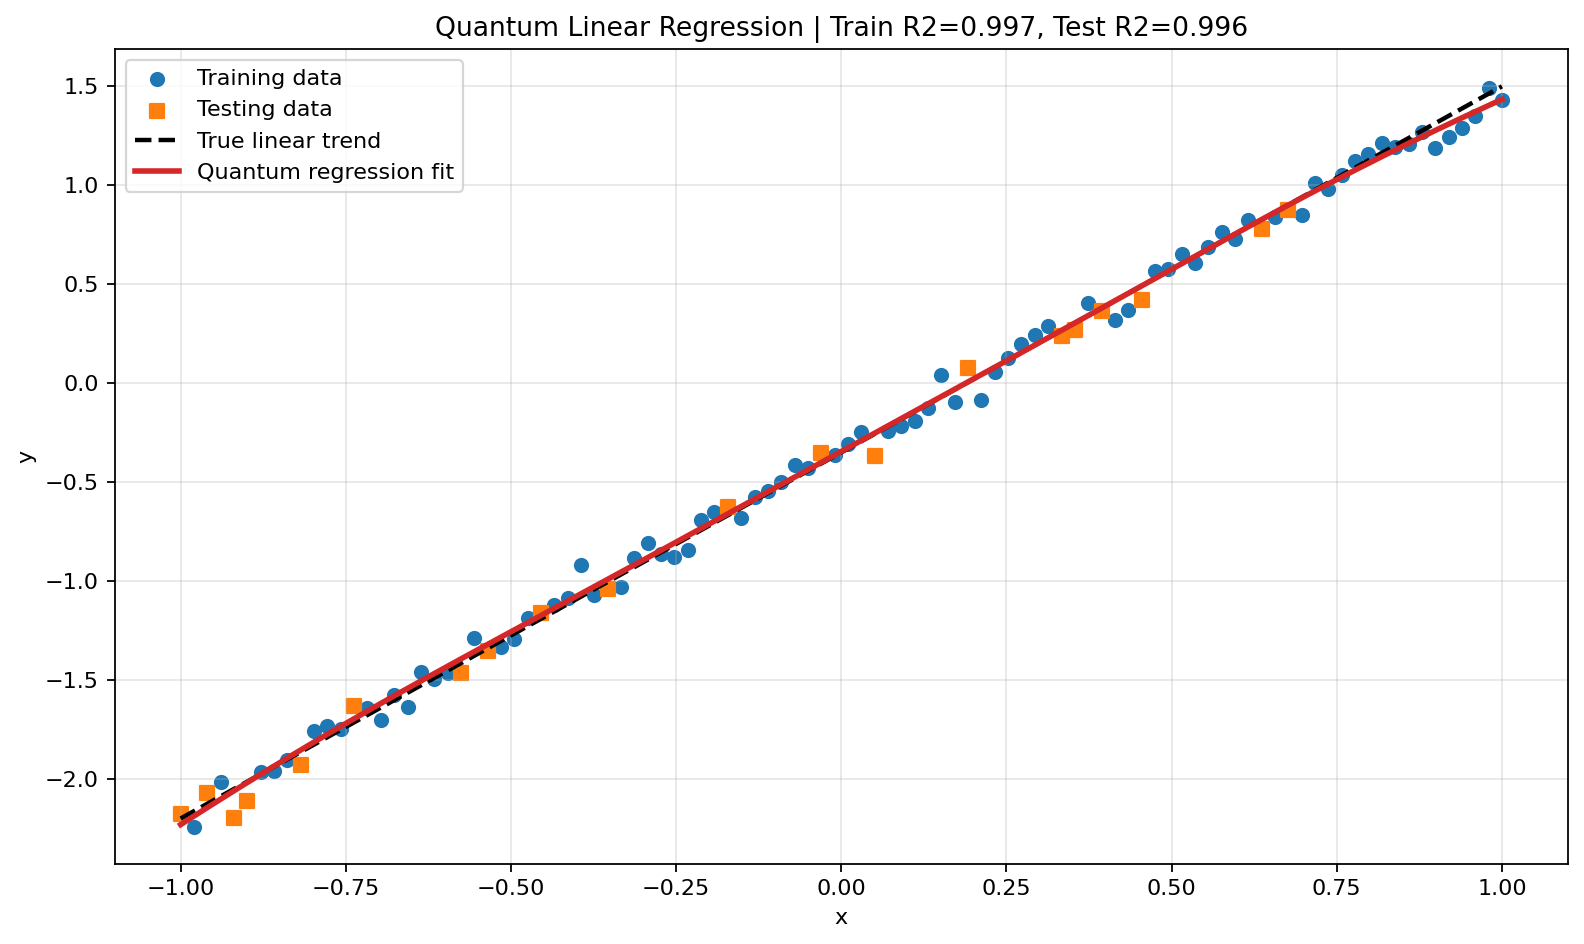
\includegraphics[width=0.92\textwidth]{figures/stage0_quantum_linear_regression.png}
\caption{Quantum linear regression on 100 generated points with an 80:20 train-test split. The quantum feature-map fit follows the true linear trend closely and generalizes well to the testing points.}
\end{figure}

\subsection{Quantum Cubic Regression}
For cubic regression, a four-qubit feature map is used. The encoded variables include $x$, $x^2$, $x^3$, and $\sin(\pi x)$, followed by an entangling ring of CNOT gates. The feature vector includes polynomial terms, local $Z$ expectations, and pairwise $ZZ$ expectations. The true curve is
\begin{equation}
    y = 0.65x^3 - 0.45x^2 + 0.85x + 0.25 + \eta .
\end{equation}
This stage demonstrates that the quantum feature map can represent nonlinear behavior without explicitly optimizing a deep neural network.

\begin{table}[H]
\centering
\caption{Stage 0 quantum cubic regression metrics.}
\begin{tabular}{lccc}
\toprule
Split & RMSE & MAE & $R^2$ \\
\midrule
Training & 0.0848 & 0.0662 & 0.9965 \\
Testing  & 0.1015 & 0.0819 & 0.9938 \\
\bottomrule
\end{tabular}
\end{table}

\begin{figure}[H]
\centering
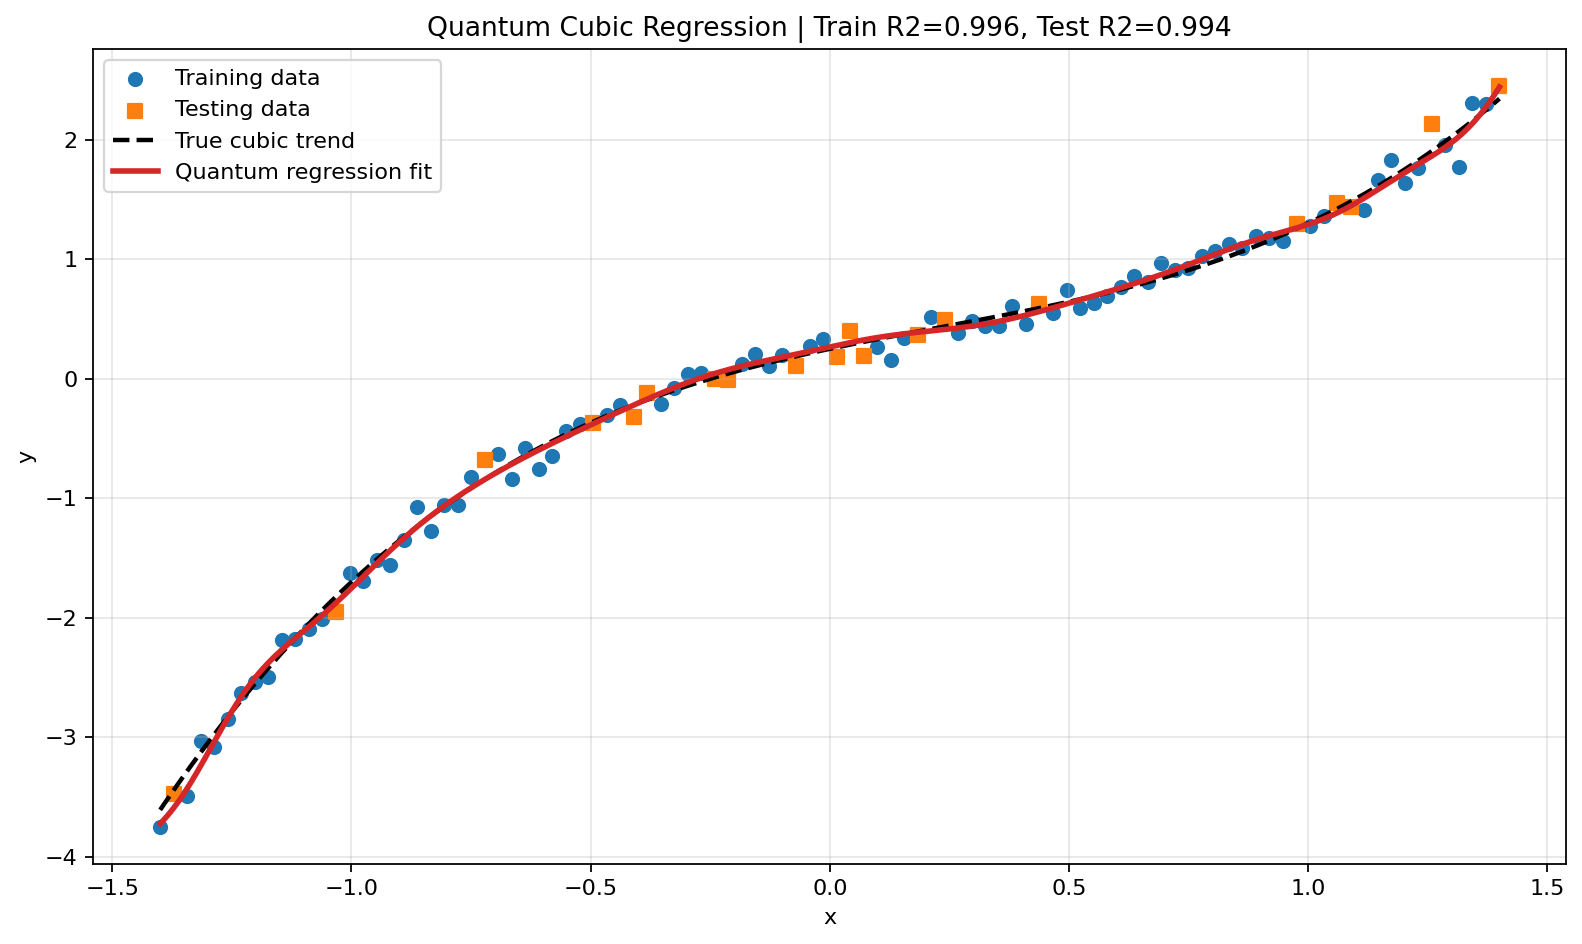
\includegraphics[width=0.92\textwidth]{figures/stage0_quantum_cubic_regression.png}
\caption{Quantum cubic regression result. The four-qubit feature map captures the nonlinear cubic trend while retaining strong testing performance.}
\end{figure}

\section{Stage 1: Synthetic Model Training and Forward Modeling}
\subsection{Geological Model}
The Stage 1 synthetic model is a 10 km profile with a 2.5 km depth extent. It contains four geological units:
\begin{itemize}
    \item \textbf{Host rock:} background unit with zero reference density contrast.
    \item \textbf{Dense body:} positive density contrast body embedded on the left side of the model.
    \item \textbf{Faulted basin:} lower-density unit on the right side, bounded by an inclined fault.
    \item \textbf{Soil layer:} thin near-surface unit affecting radiometric response.
\end{itemize}
The forward model generates gravity and radiometric observations. Gravity is computed from the discretized prism model. Radiometric responses are generated from assigned K, U, and Th values mixed with the soil response.

\subsection{Inversion Parameters}
The synthetic inversion solves for four physical parameters:
\begin{enumerate}
    \item fault position $x_f$,
    \item dense-body density contrast $\rho_d$,
    \item basin-density contrast $\rho_b$,
    \item dense-body top depth $z_d$.
\end{enumerate}
In the quantum ansatz, these are decoded from expectation values of an 8-qubit, 4-layer circuit. Latin Hypercube Sampling is used for multi-start diversity. Monte Carlo perturbation is used to estimate uncertainty.

\begin{figure}[H]
\centering
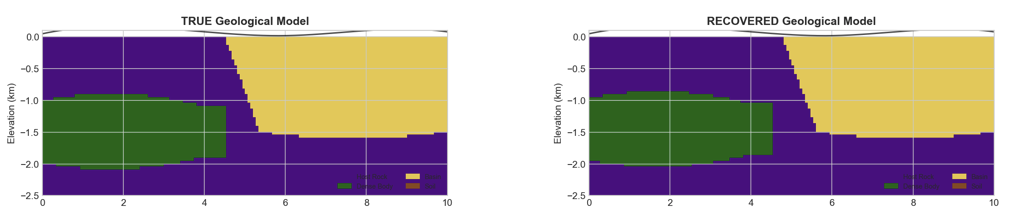
\includegraphics[width=0.95\textwidth]{figures/stage1_true_recovered_geology.png}
\caption{Stage 1 synthetic true and recovered geological sections. The recovered model reproduces the dense body, basin edge, and main fault geometry.}
\end{figure}

\begin{figure}[H]
\centering
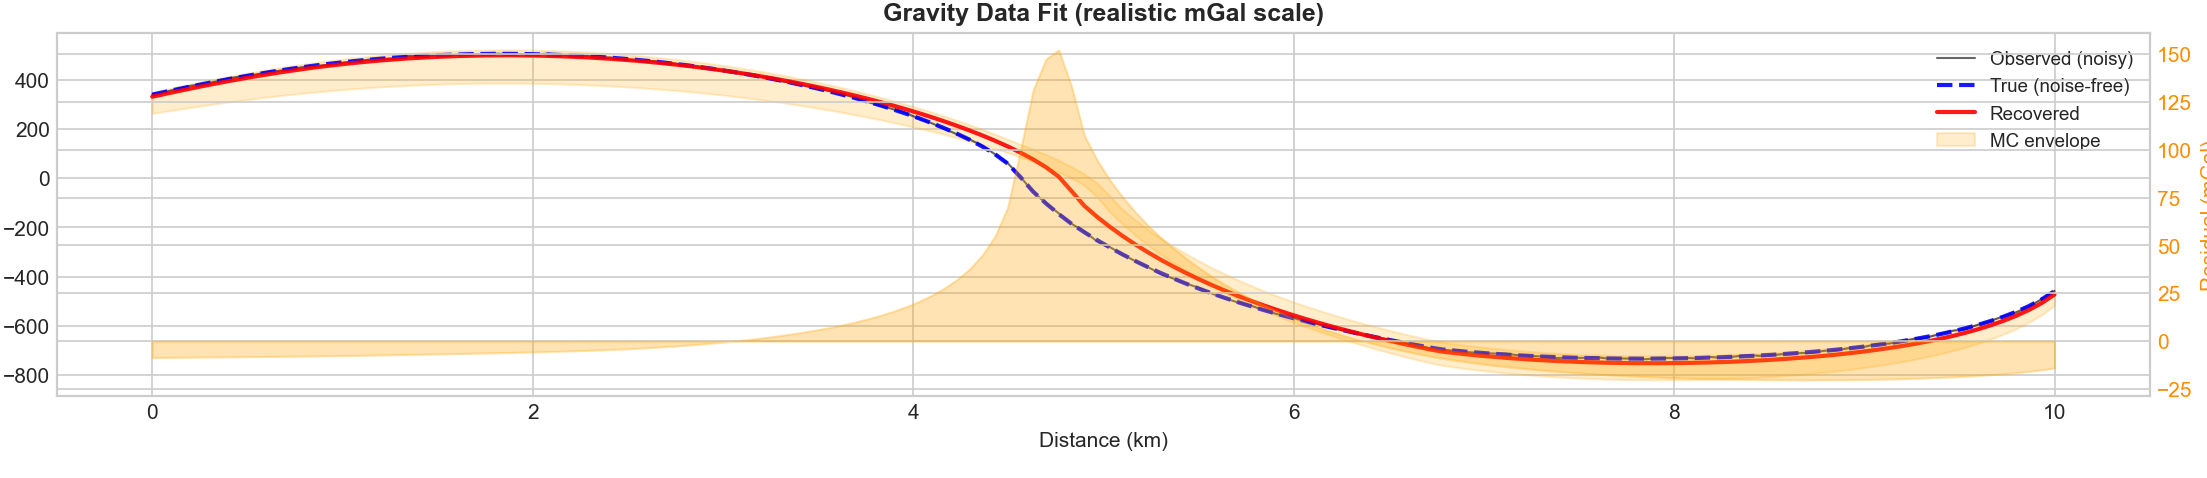
\includegraphics[width=0.95\textwidth]{figures/stage1_synthetic_gravity_fit.png}
\caption{Stage 1 synthetic gravity response. The recovered response follows the true/noisy gravity anomaly over the 10 km profile.}
\end{figure}

\begin{figure}[H]
\centering
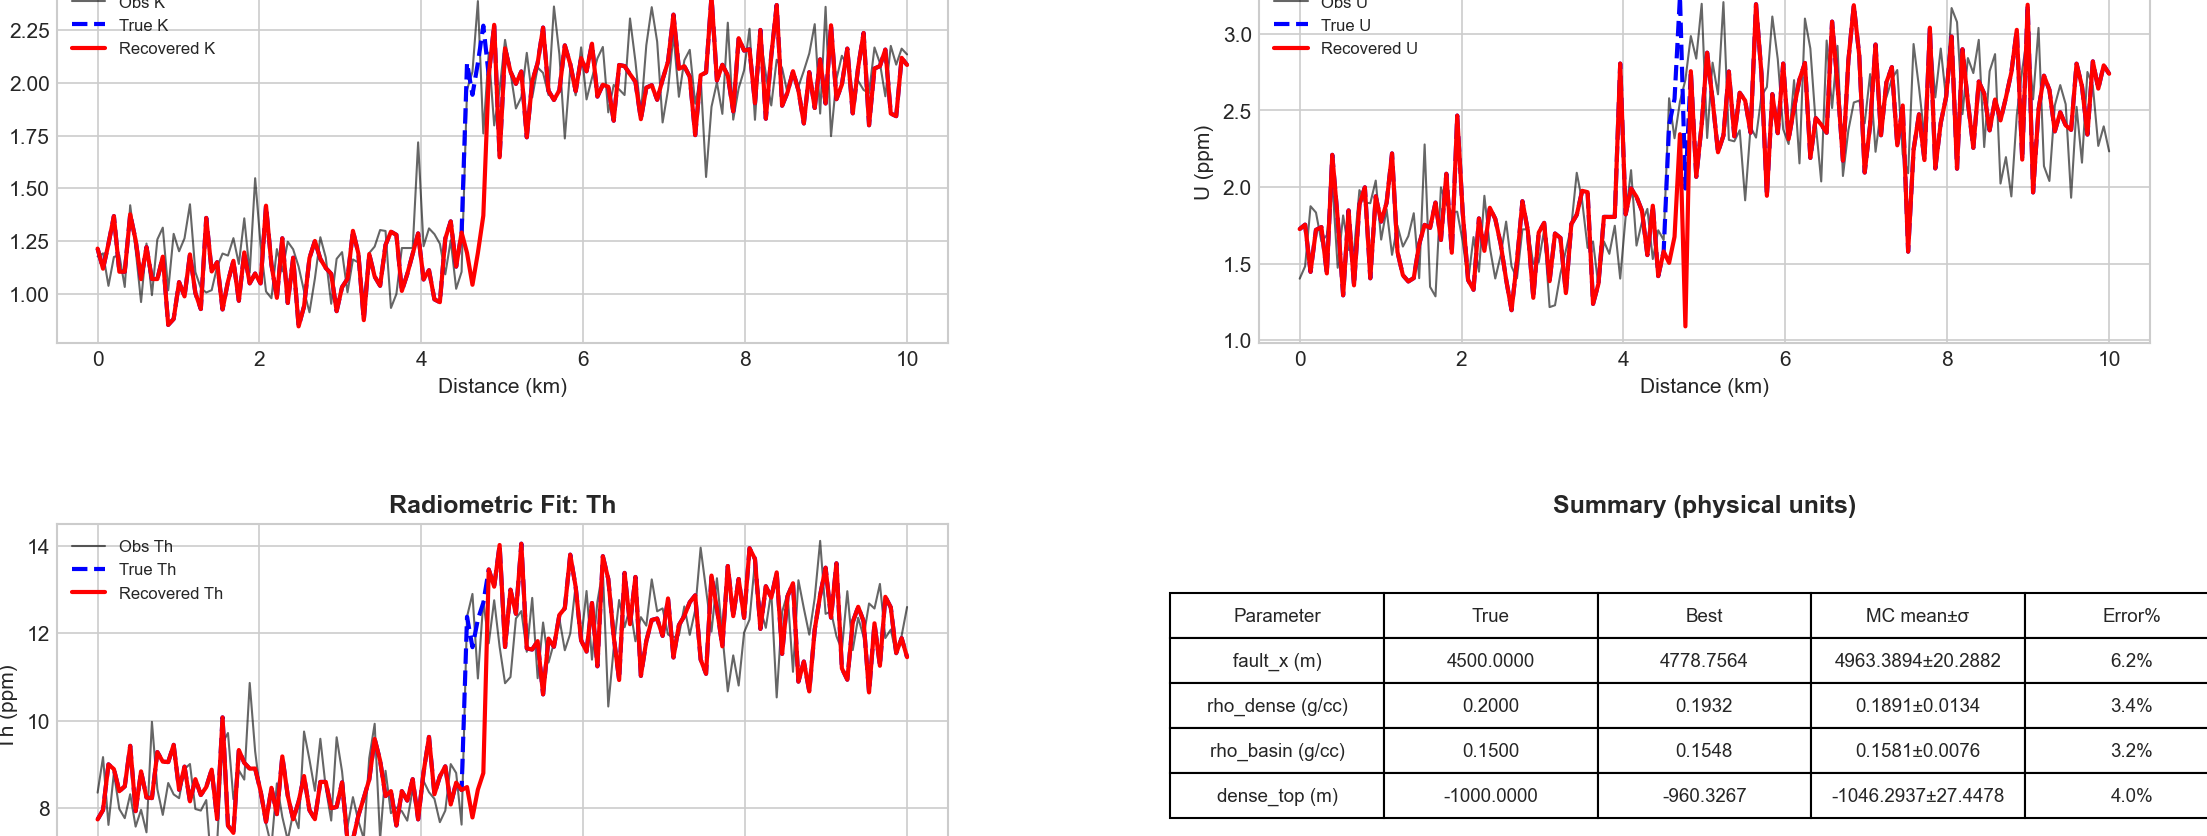
\includegraphics[width=\textwidth]{figures/stage1_synthetic_radiometric_fits.png}
\caption{Stage 1 synthetic K, U, and Th radiometric fits. The radiometric channels constrain the near-surface side of the geological contact.}
\end{figure}

\begin{table}[H]
\centering
\caption{Stage 1 synthetic parameter recovery.}
\begin{tabular}{lccc}
\toprule
Parameter & True & Best recovered & Error \\
\midrule
Fault position & 4500 m & 4778.8 m & 6.2\% \\
Dense contrast & 0.200 g/cc & 0.193 g/cc & 3.4\% \\
Basin contrast & 0.150 g/cc & 0.155 g/cc & 3.2\% \\
Dense top depth & -1000 m & -960 m & 4.0\% \\
\bottomrule
\end{tabular}
\end{table}

\begin{figure}[H]
\centering
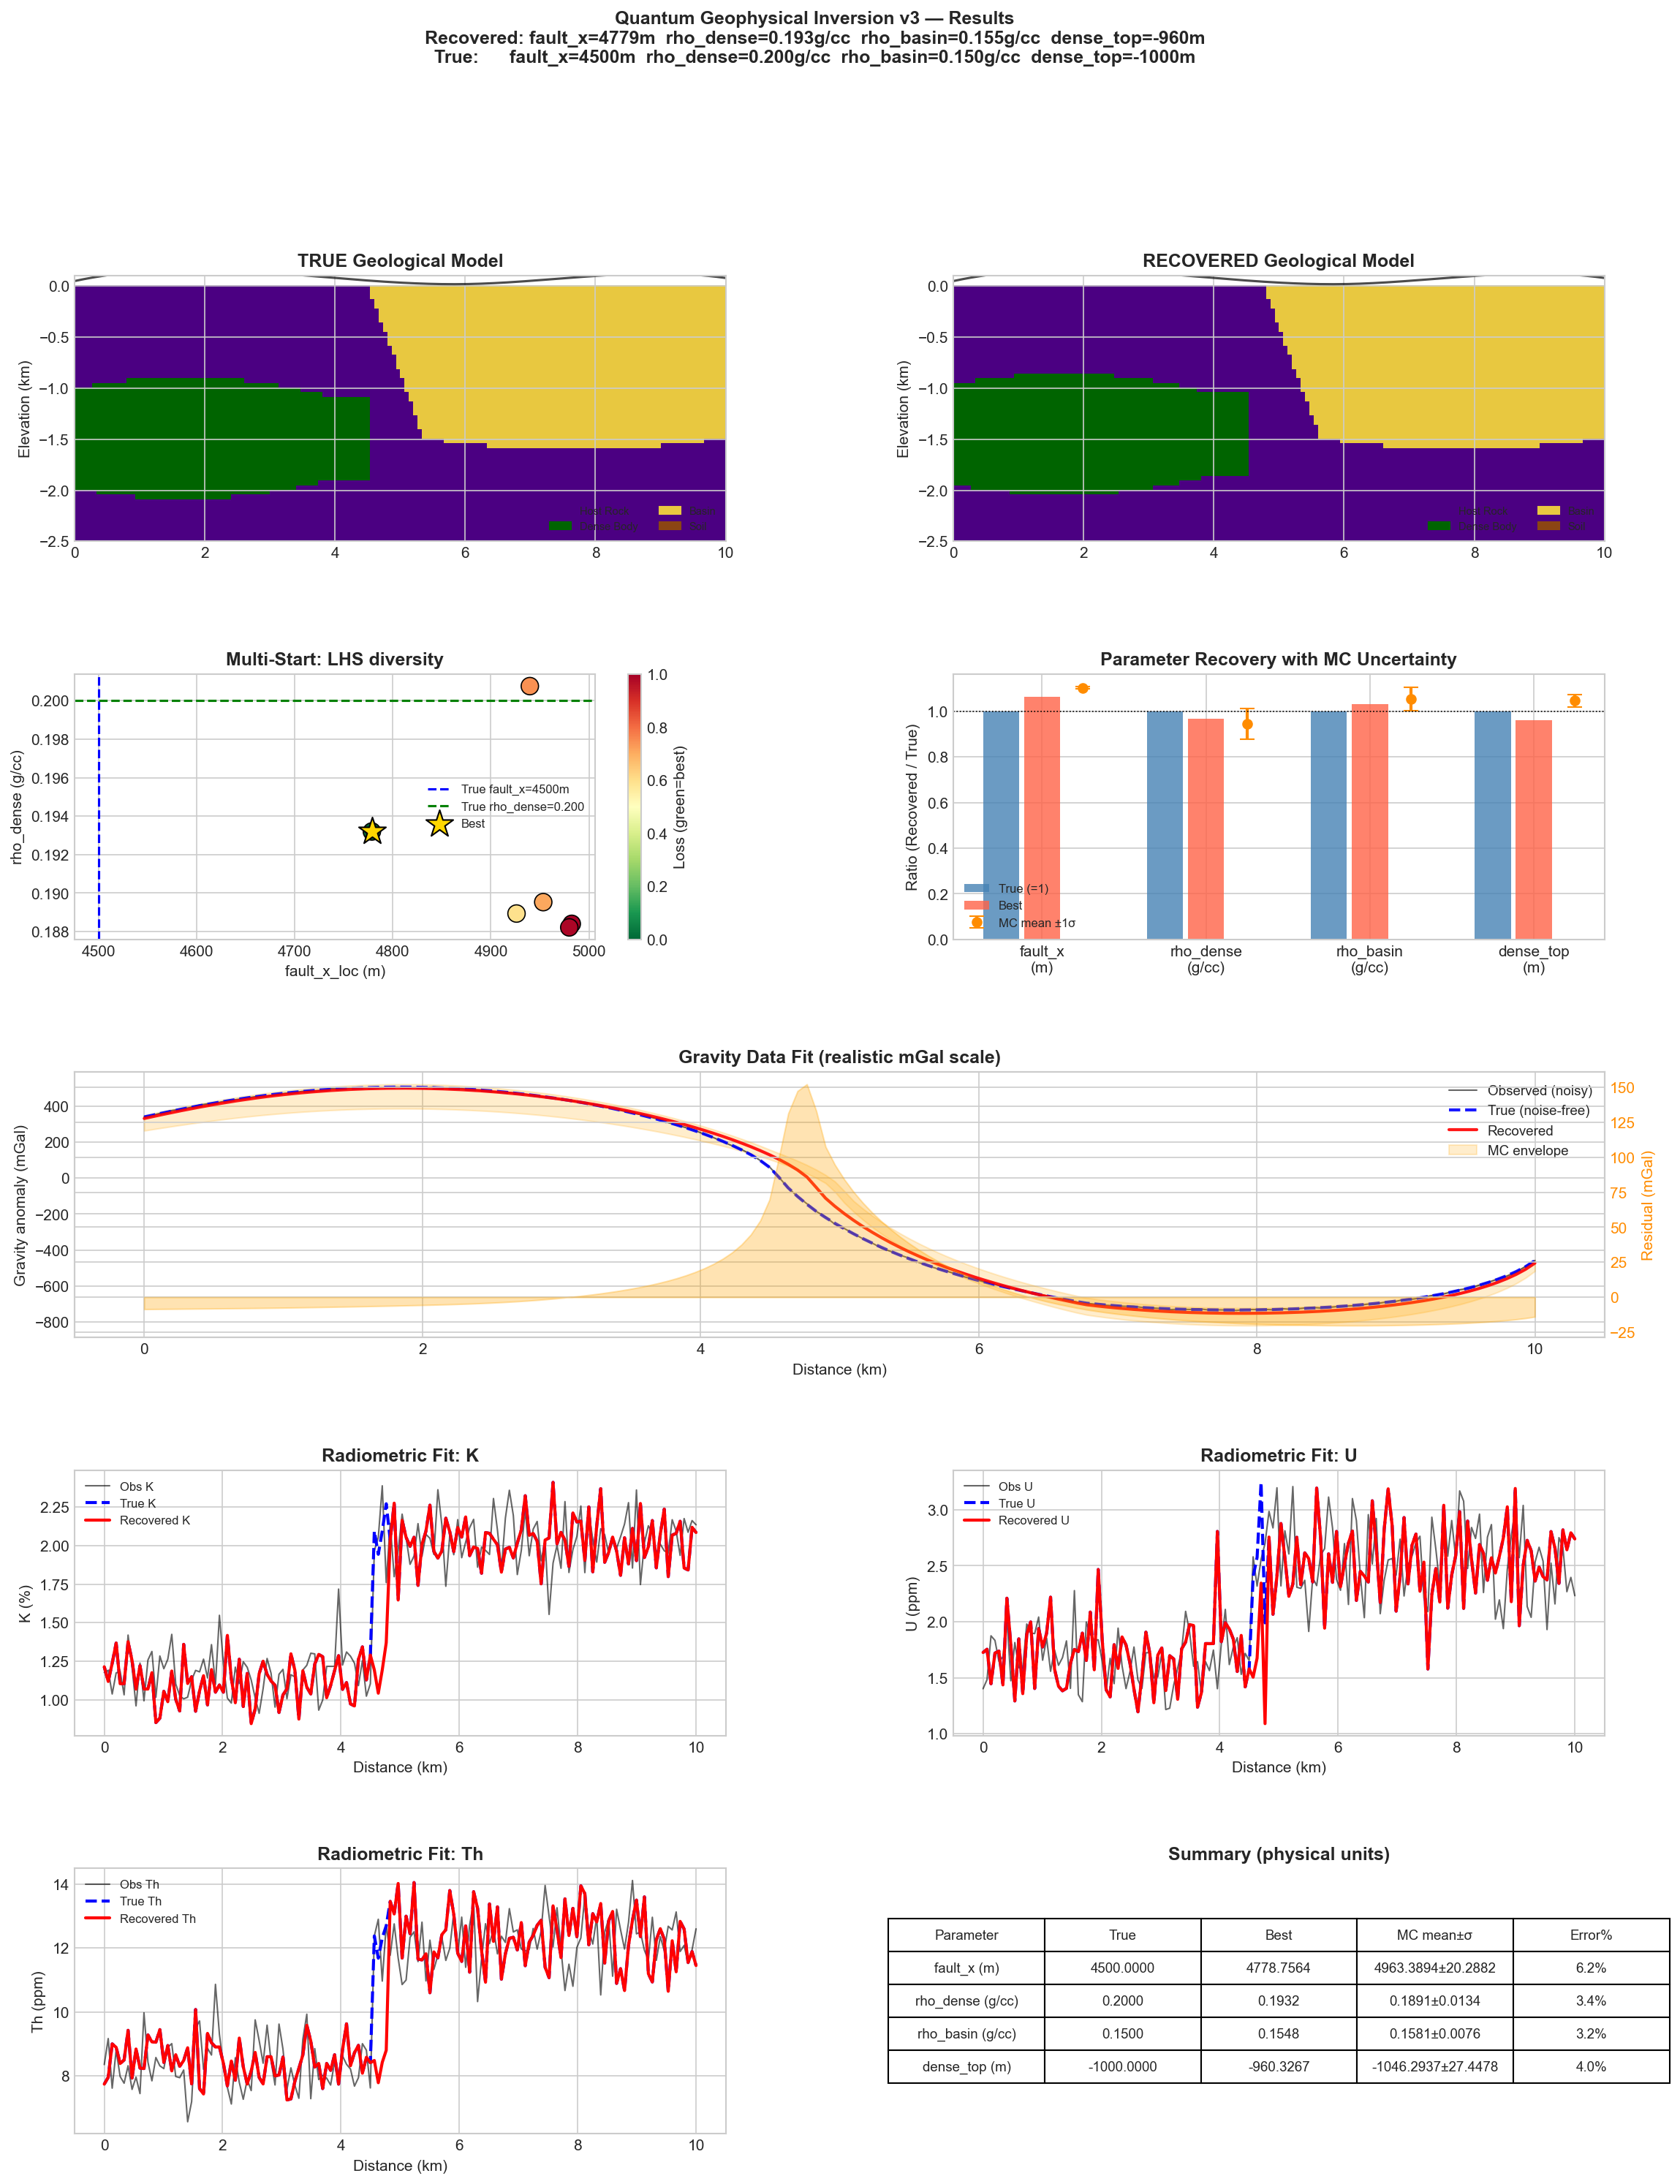
\includegraphics[width=\textwidth]{figures/stage1_training_results_v3.png}
\caption{Complete Stage 1 synthetic inversion result page.}
\end{figure}

\section{Stage 2: Real Data Testing on a 10 km Window}
\subsection{Need for Real-Data Calibration}
The first attempt to apply the synthetic inversion directly to real data was unsatisfactory because it assumed that synthetic gravity amplitude, sign, and radiometric scaling were directly comparable to the field measurements. Real Bouguer gravity includes a regional component, possible profile-polarity mismatch, survey offsets, and field noise. Real radiometric values may also reflect surface enrichment, weathering, soil cover, and acquisition effects. Therefore, the real-data workflow introduces:
\begin{itemize}
    \item robust polynomial regional-trend removal from Bouguer gravity,
    \item automatic 10 km window selection,
    \item optional profile reversal,
    \item linear scale-offset calibration for gravity and each radiometric channel,
    \item real-style radiometric enrichment terms,
    \item Monte Carlo uncertainty estimation.
\end{itemize}

\subsection{Preprocessing}
The 30 km real profile is first fitted with a robust degree-2 regional trend. The residual anomaly is used as the inversion target. K, U, and Th values are smoothed with a Savitzky-Golay filter after resampling to the model grid. The selected 10 km window is mapped into the 0--10 km local model coordinate system.

\begin{figure}[H]
\centering
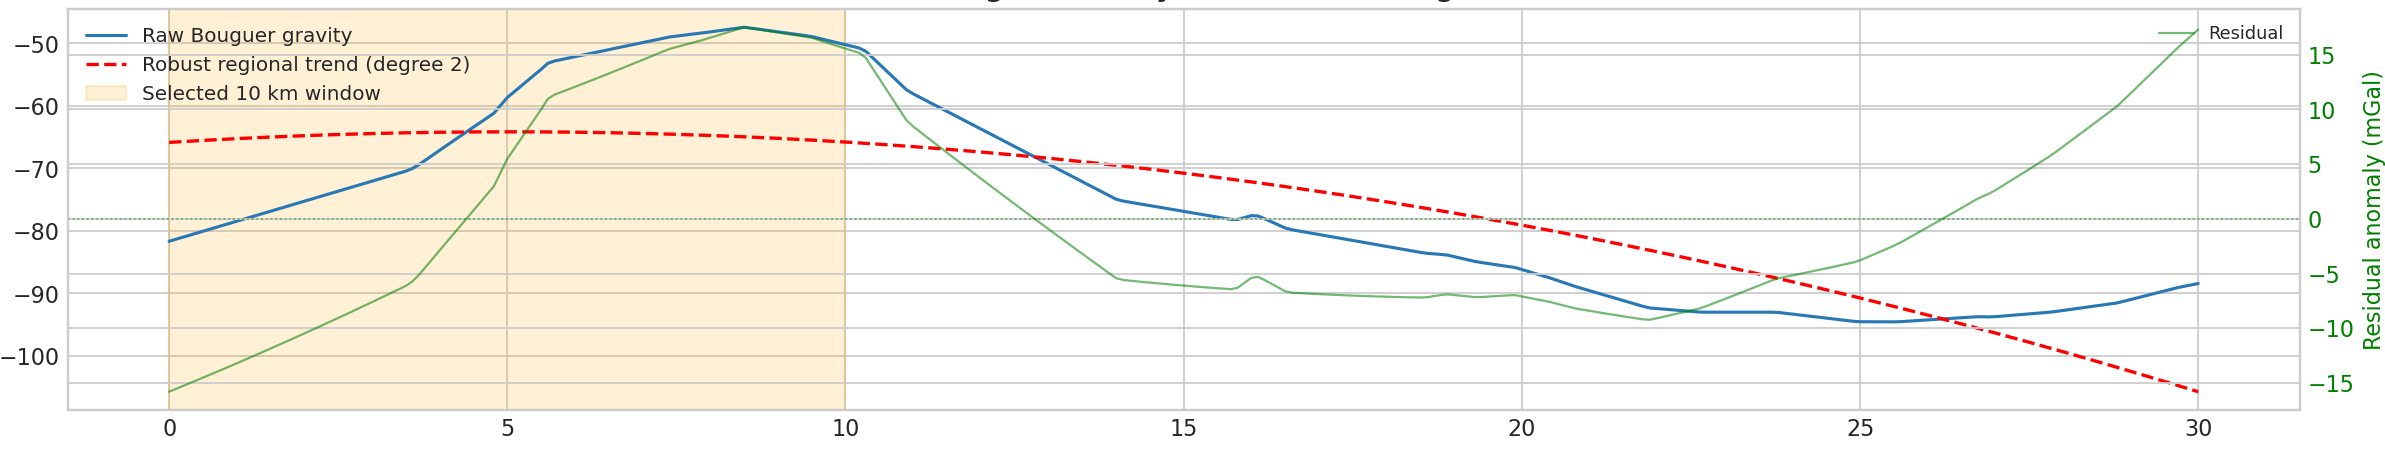
\includegraphics[width=0.95\textwidth]{figures/stage2_real_full_profile_trend.png}
\caption{Full real Bouguer gravity profile and removed regional trend for the 10 km real-data inversion stage.}
\end{figure}

\subsection{Recovered 10 km Model}
The best 10 km inversion selected the 0--10 km window without profile reversal. The recovered model indicates a fault near 1.50 km in local model coordinates, an effective dense-body contrast of 0.282 g/cc, basin contrast of 0.0398 g/cc, and dense-body top depth near -2253 m. These contrasts should be interpreted as calibrated effective contrasts rather than direct laboratory-density estimates.

\begin{figure}[H]
\centering
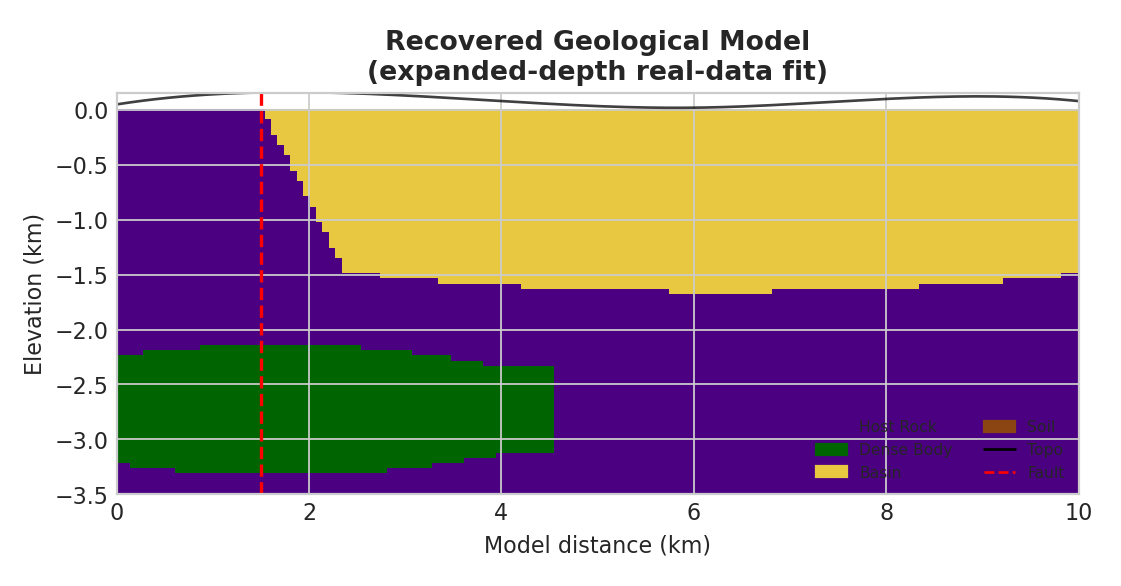
\includegraphics[width=0.85\textwidth]{figures/stage2_real_recovered_geology.png}
\caption{Recovered geological section for the best 10 km real-data inversion.}
\end{figure}

\begin{figure}[H]
\centering
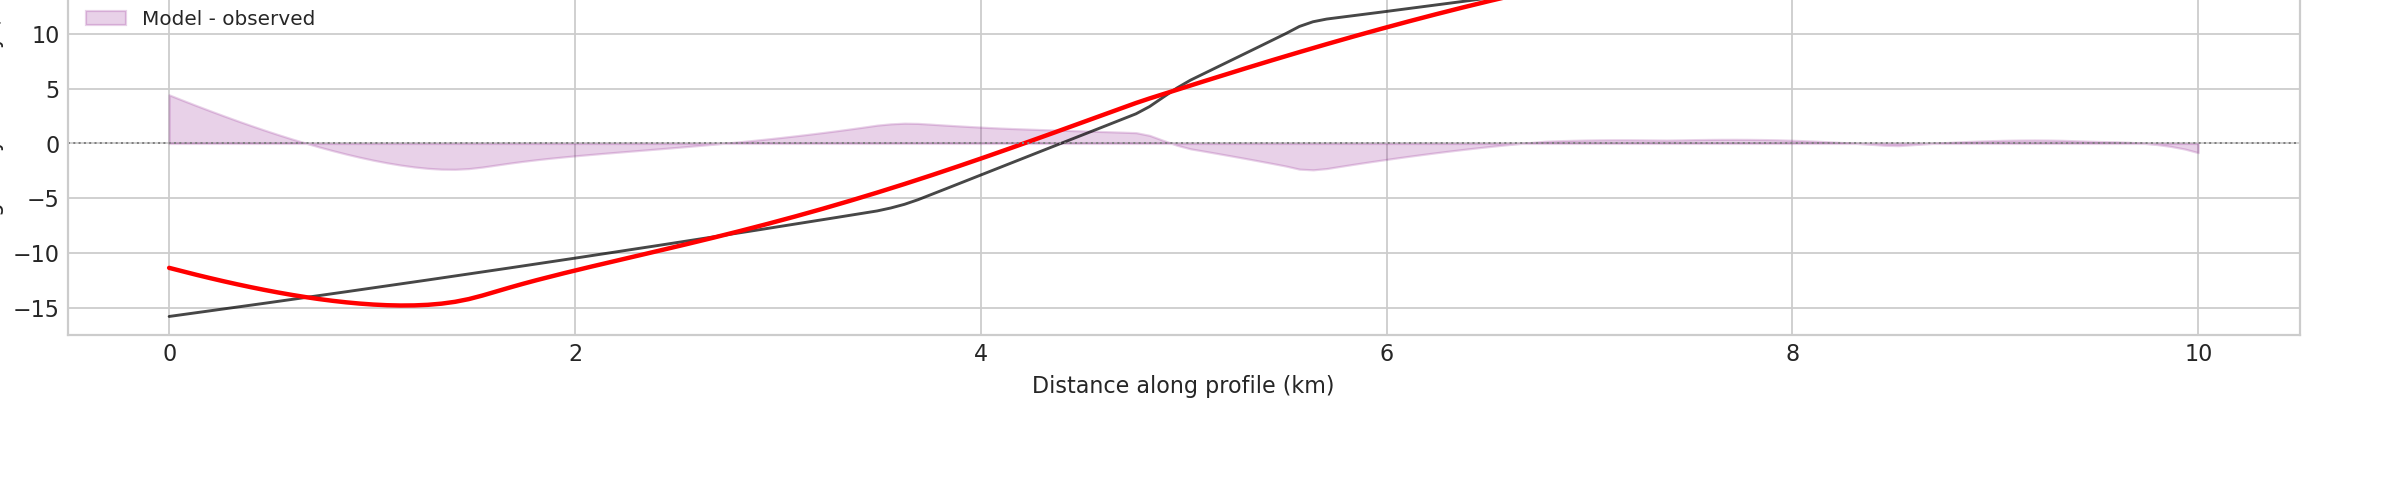
\includegraphics[width=0.95\textwidth]{figures/stage2_real_gravity_fit.png}
\caption{Stage 2 gravity fit for the selected 10 km real-data window. The calibrated gravity response reaches $R^2=0.989$ and RMSE $=1.267$ mGal.}
\end{figure}

\begin{figure}[H]
\centering
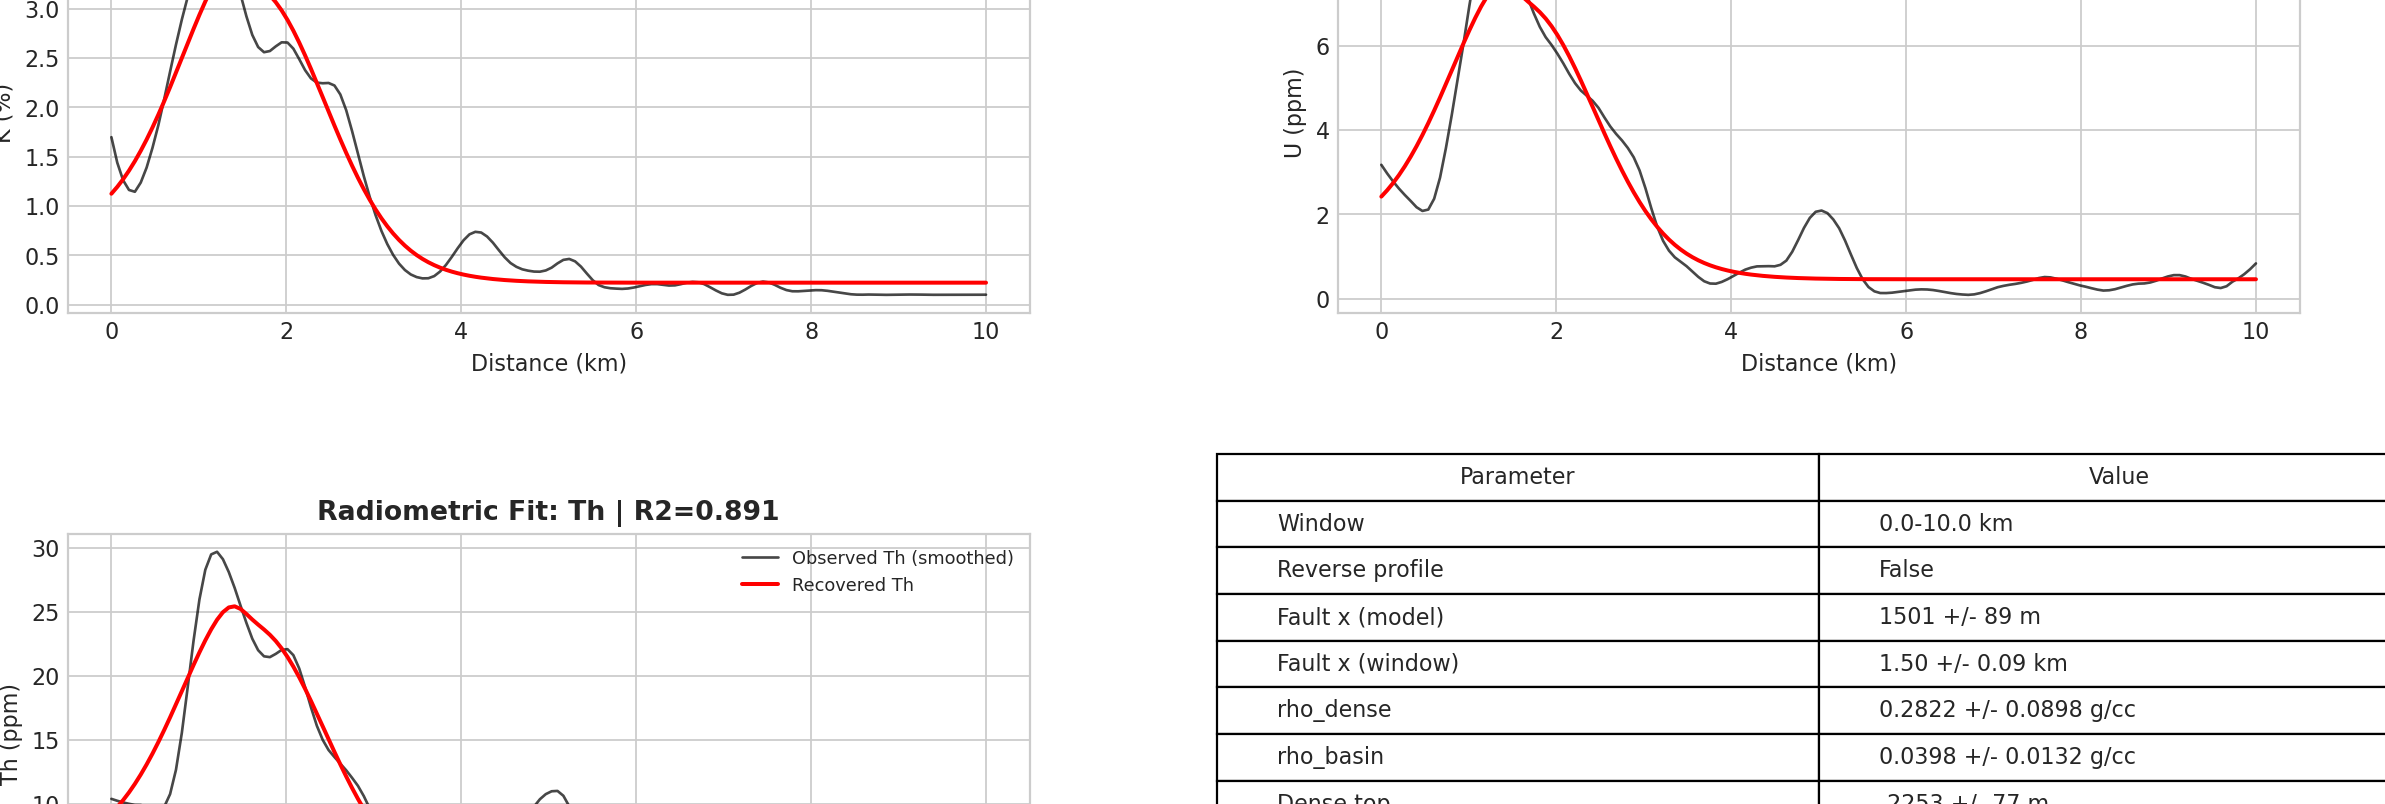
\includegraphics[width=\textwidth]{figures/stage2_real_radiometric_fits.png}
\caption{Stage 2 K, U, and Th fits for the best 10 km real-data inversion.}
\end{figure}

\begin{table}[H]
\centering
\caption{Stage 2 real-data 10 km inversion summary.}
\begin{tabular}{lc}
\toprule
Quantity & Value \\
\midrule
Selected window & 0--10 km \\
Profile reversed & False \\
Best loss & 0.04865 \\
Fault position & 1500.8 m \\
Dense-body contrast & 0.2822 g/cc \\
Basin contrast & 0.0398 g/cc \\
Dense top depth & -2253 m \\
Gravity $R^2$ / RMSE & 0.989 / 1.267 mGal \\
K $R^2$ / RMSE & 0.951 / 0.238 \\
U $R^2$ / RMSE & 0.929 / 0.633 \\
Th $R^2$ / RMSE & 0.891 / 2.541 \\
\bottomrule
\end{tabular}
\end{table}

\begin{figure}[H]
\centering
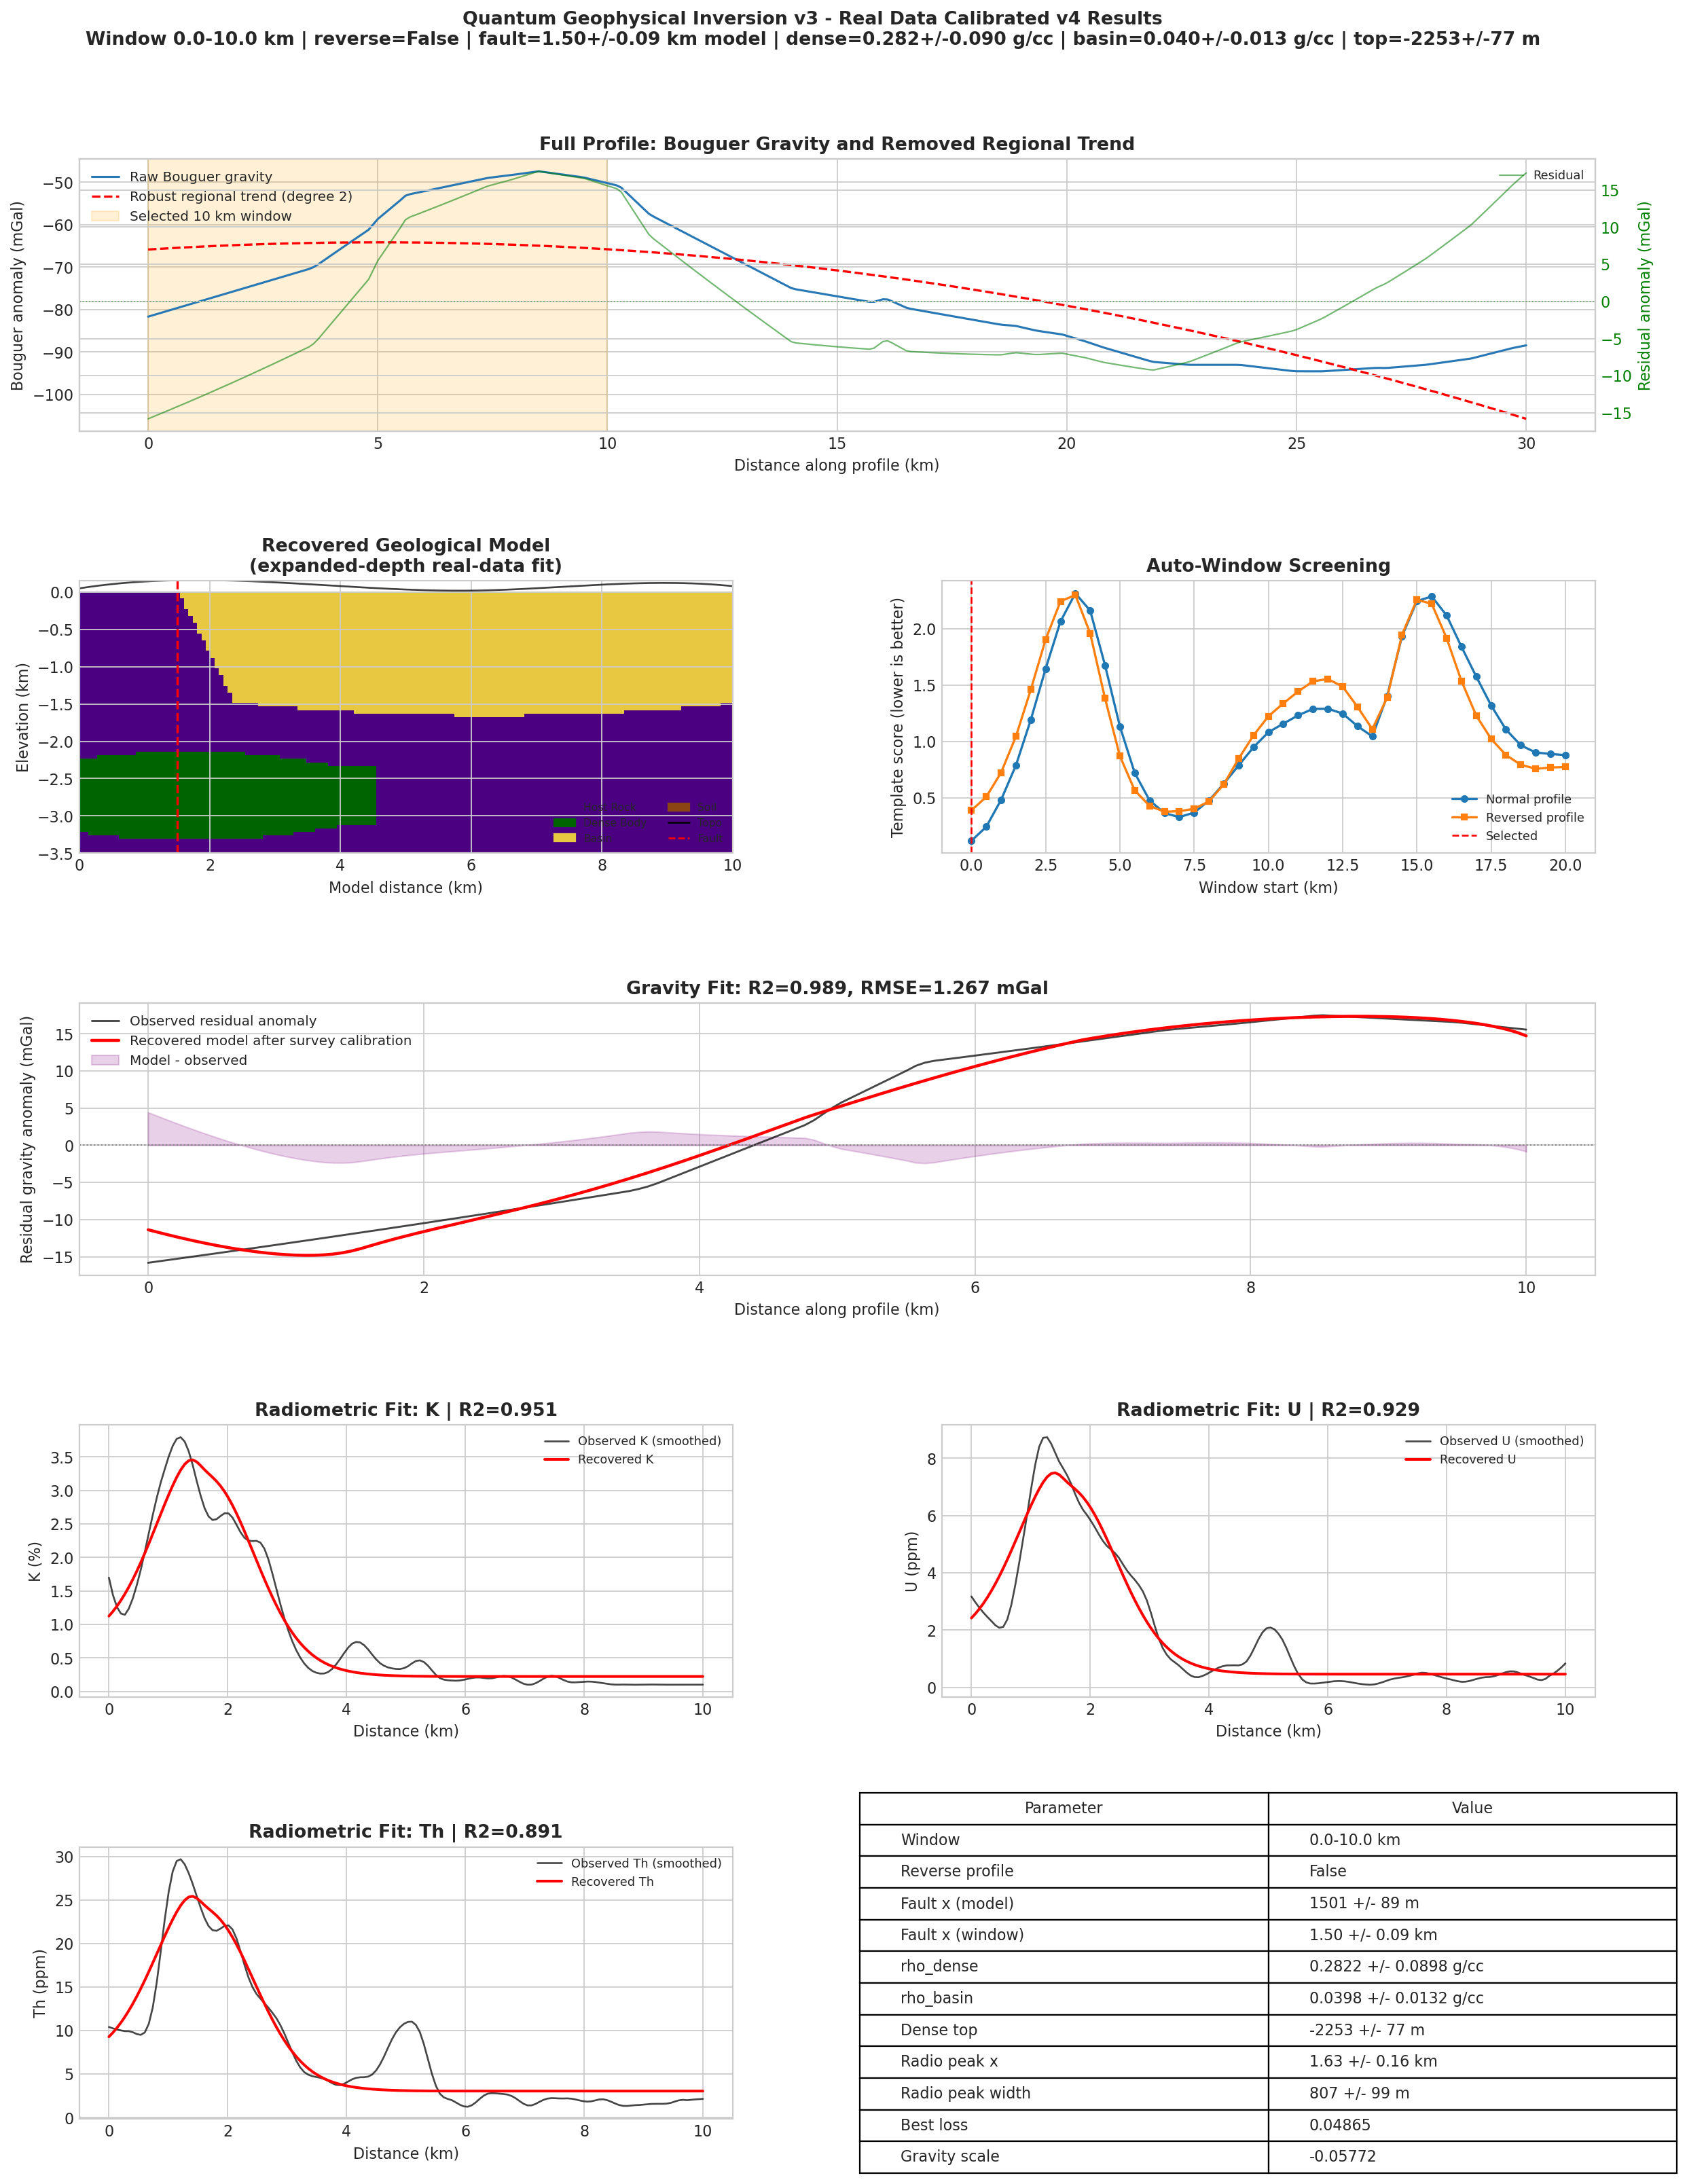
\includegraphics[width=\textwidth]{figures/stage2_real_data_best_plot.png}
\caption{Complete Stage 2 10 km real-data inversion result page.}
\end{figure}

\section{Stage 3: Full 30 km Profile Through Three-Window Stitching}
\subsection{Motivation}
The real-data forward model is a 10 km local model. Extending it directly to 30 km would require a new globally coupled geometry, additional regularization, and careful treatment of regional field separation across the entire line. Instead, Stage 3 applies the validated 10 km inversion independently to three windows: 0--10 km, 10--20 km, and 20--30 km. The three local geological interpretations are then stitched into one full-profile display.

This approach is feasible as a stitched interpretation but should not be described as a single global inversion. Each window has its own residual data, calibration coefficients, local coordinates, and boundary behavior. Discontinuities near 10 km and 20 km are therefore treated as calibration/window artifacts unless independently supported by geology.

\begin{figure}[H]
\centering
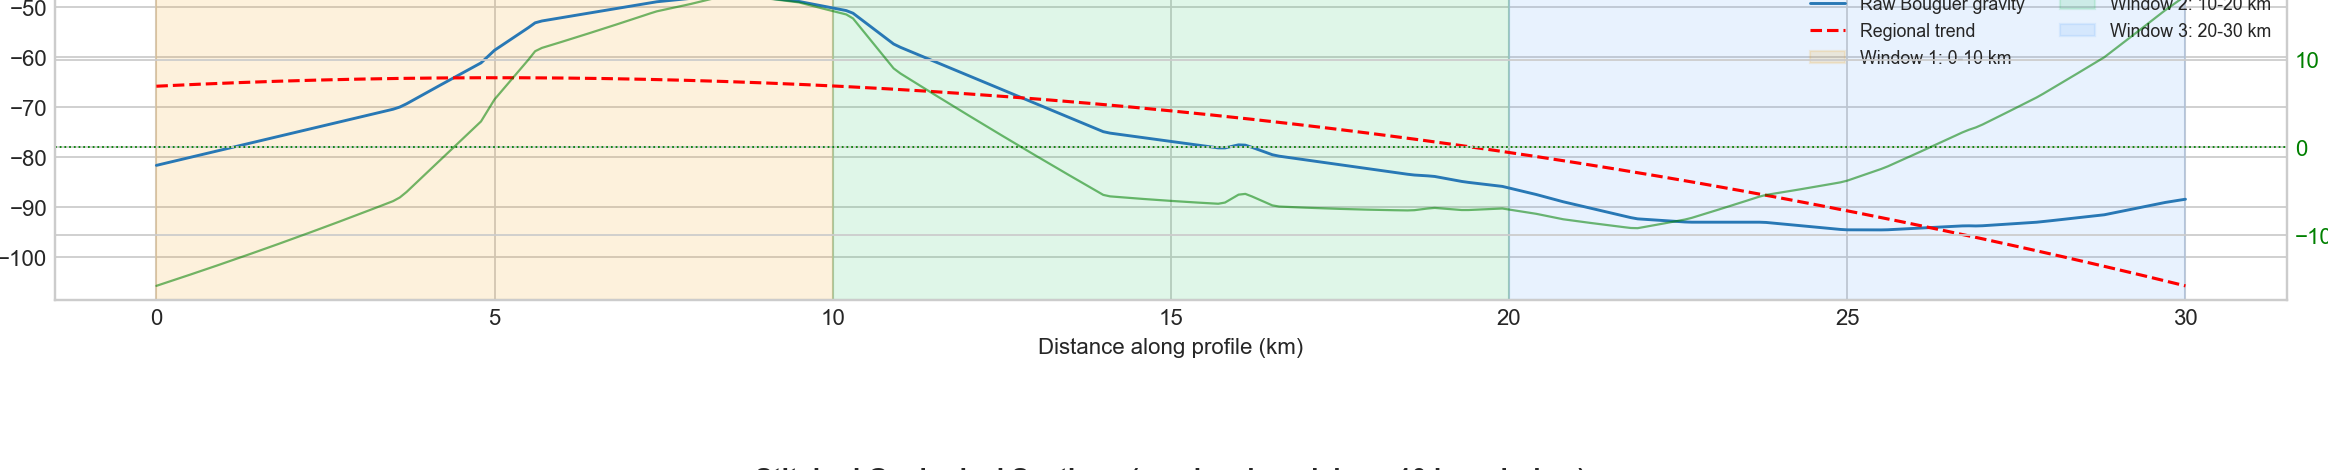
\includegraphics[width=0.95\textwidth]{figures/stage3_full_profile_trend.png}
\caption{Full 30 km Bouguer profile with three inversion windows and the regional trend.}
\end{figure}

\subsection{Stitched Geological Interpretation}
The stitched geological section shows three local models arranged along the full 30 km distance axis. The main interpreted fault locations are near 3.25 km, 11.54 km, and 28.33 km. The third window is reversed during fitting, indicating that the local anomaly orientation is better matched by reversing the model coordinate direction.

\begin{figure}[H]
\centering
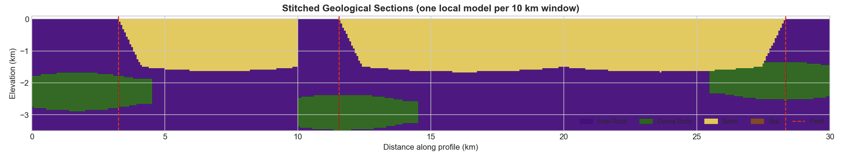
\includegraphics[width=\textwidth]{figures/stage3_stitched_geology.png}
\caption{Stage 3 stitched geological section across the 30 km profile. Each 10 km section is independently inverted and then placed in global distance coordinates.}
\end{figure}

\begin{figure}[H]
\centering
\begin{subfigure}{0.98\textwidth}
\centering
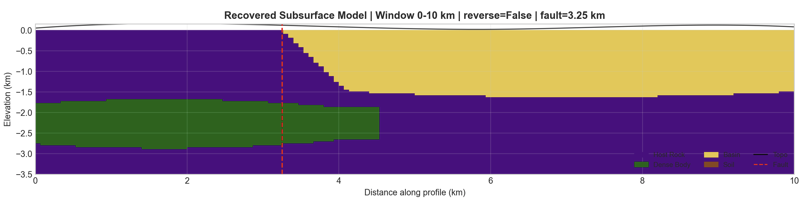
\includegraphics[width=\textwidth]{figures/stage3_window_00_10_geology.png}
\caption{Window 1: 0--10 km.}
\end{subfigure}

\begin{subfigure}{0.98\textwidth}
\centering
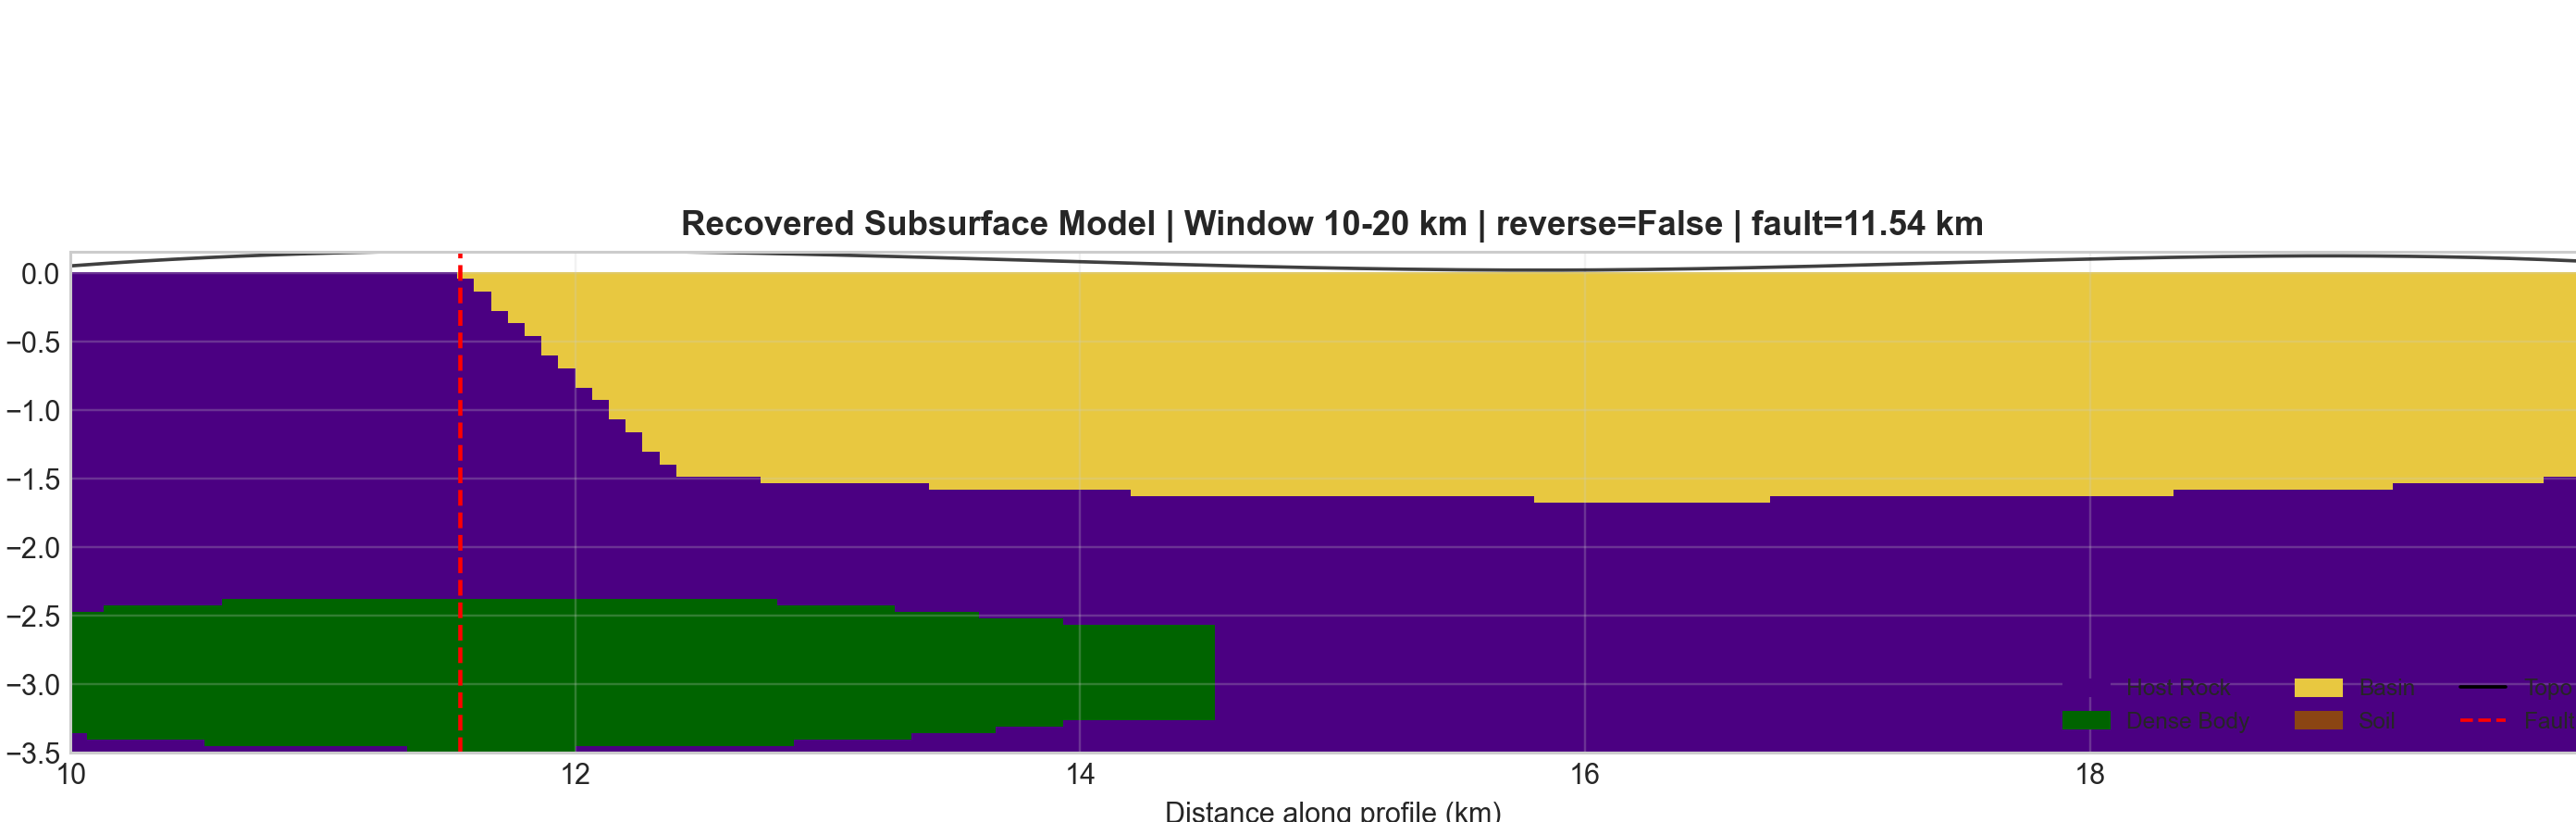
\includegraphics[width=\textwidth]{figures/stage3_window_10_20_geology.png}
\caption{Window 2: 10--20 km.}
\end{subfigure}

\begin{subfigure}{0.98\textwidth}
\centering
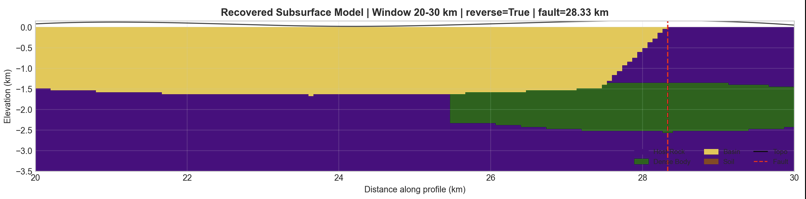
\includegraphics[width=\textwidth]{figures/stage3_window_20_30_geology.png}
\caption{Window 3: 20--30 km.}
\end{subfigure}
\caption{Individual recovered geological/subsurface profiles for all three Stage 3 windows.}
\end{figure}

\subsection{Unified Data Fit}
The stitched gravity response reaches $R^2=0.965$ with RMSE $=1.756$ mGal. The stitched radiometric fits reach $R^2=0.883$, $0.876$, and $0.866$ for K, U, and Th respectively. The radiometric performance is lower than the single-window best case because the full profile includes multiple localized peaks and different shallow response regimes, but the fit is still strong enough to support the stitched interpretation.

\begin{figure}[H]
\centering
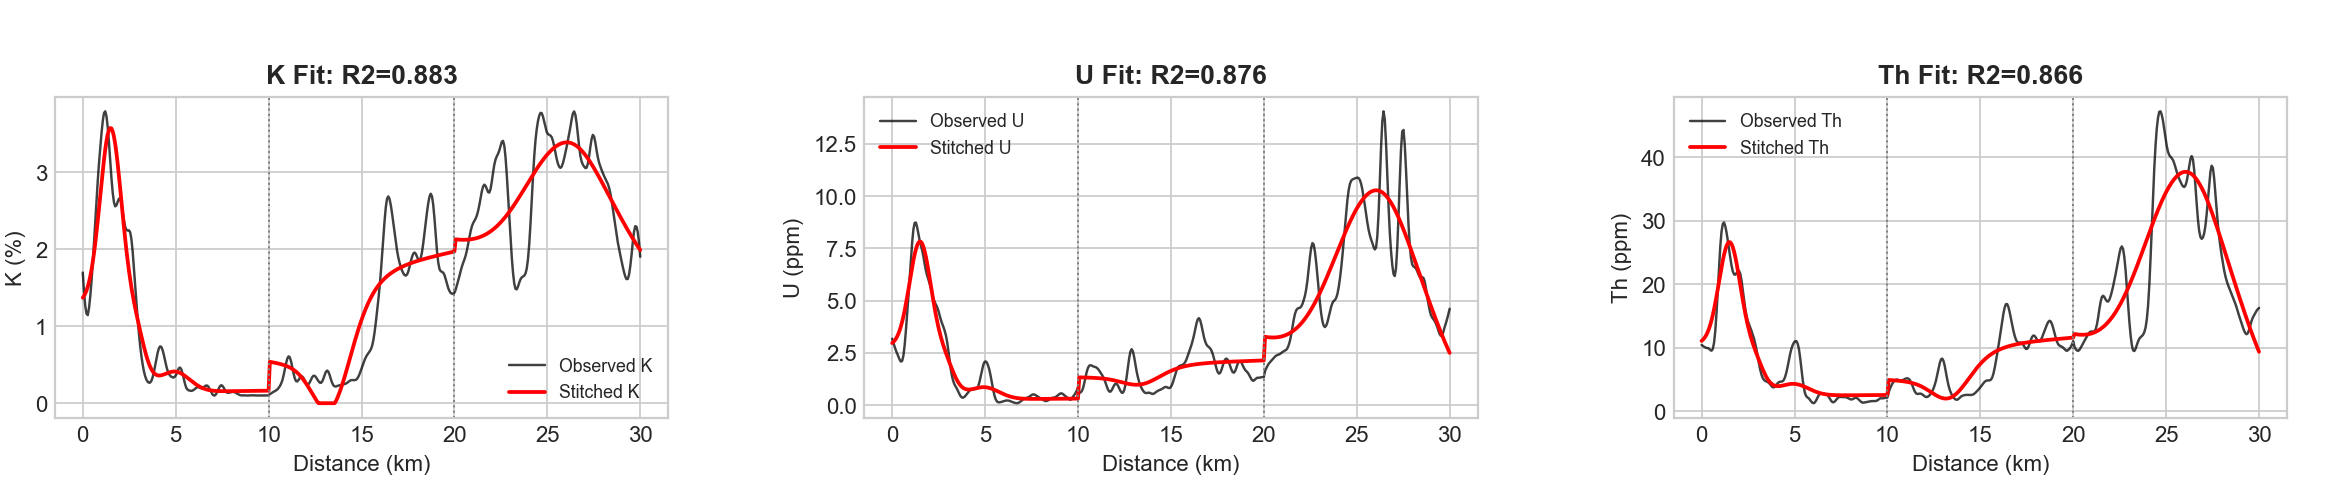
\includegraphics[width=\textwidth]{figures/stage3_unified_gravity_fit.png}
\caption{Unified Stage 3 gravity fit across the full 30 km profile.}
\end{figure}

\begin{figure}[H]
\centering
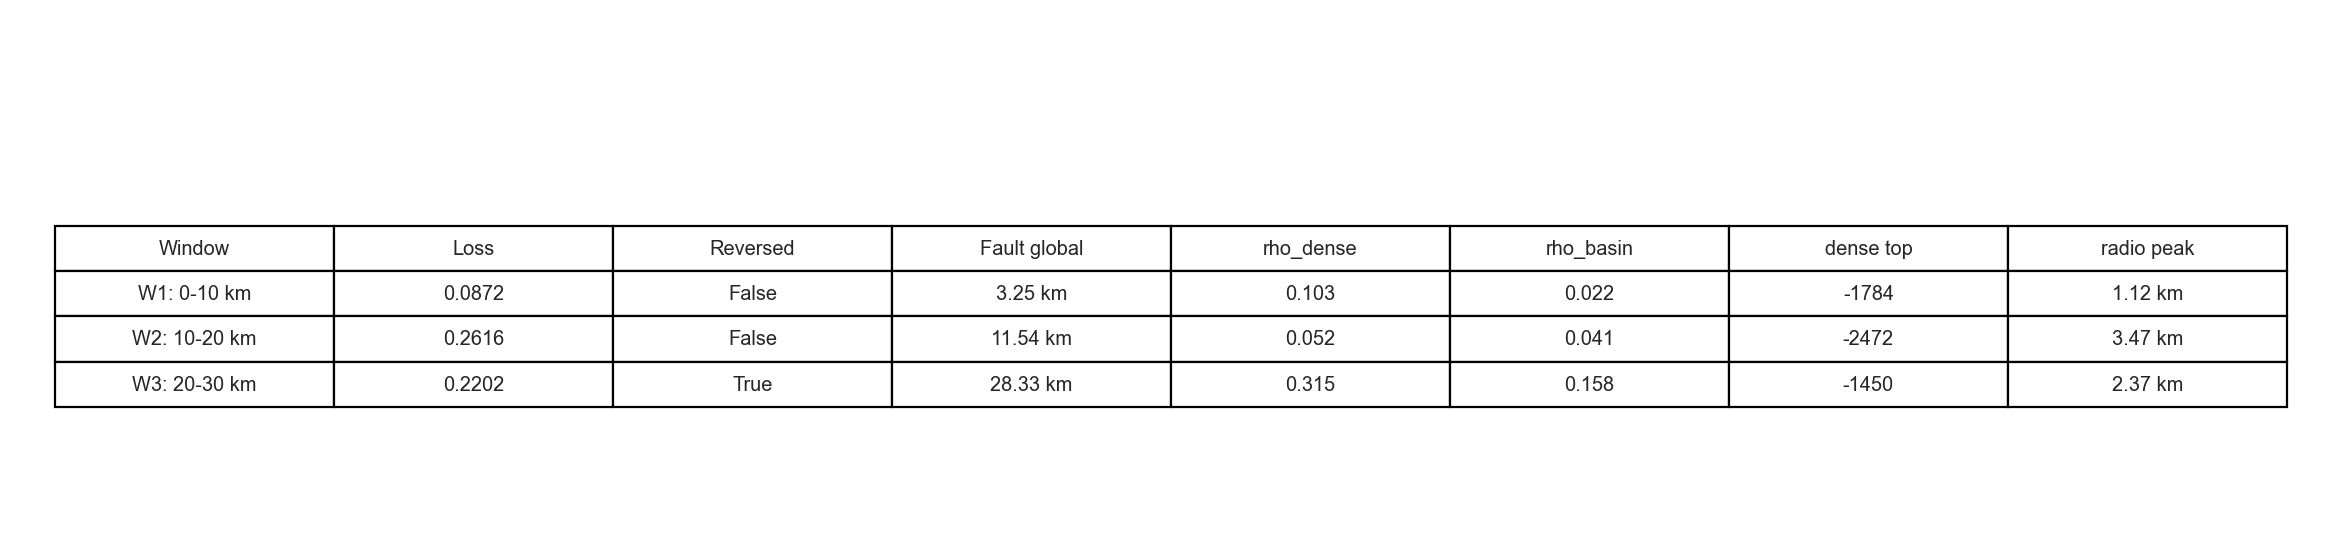
\includegraphics[width=\textwidth]{figures/stage3_unified_radiometric_fits.png}
\caption{Unified Stage 3 radiometric fits for K, U, and Th.}
\end{figure}

\begin{table}[H]
\centering
\caption{Stage 3 full-profile stitched inversion metrics.}
\begin{tabular}{lc}
\toprule
Metric & Value \\
\midrule
Unified gravity $R^2$ & 0.9650 \\
Unified gravity RMSE & 1.7556 mGal \\
Unified K $R^2$ & 0.8832 \\
Unified U $R^2$ & 0.8764 \\
Unified Th $R^2$ & 0.8663 \\
\bottomrule
\end{tabular}
\end{table}

\begin{table}[H]
\centering
\caption{Stage 3 recovered window parameters.}
\begin{tabular}{lcccccc}
\toprule
Window & Loss & Reversed & Fault & $\rho_d$ & $\rho_b$ & Dense top \\
\midrule
0--10 km & 0.0872 & False & 3.25 km & 0.103 & 0.022 & -1784 m \\
10--20 km & 0.2616 & False & 11.54 km & 0.052 & 0.041 & -2472 m \\
20--30 km & 0.2202 & True & 28.33 km & 0.315 & 0.158 & -1450 m \\
\bottomrule
\end{tabular}
\end{table}

\begin{figure}[H]
\centering
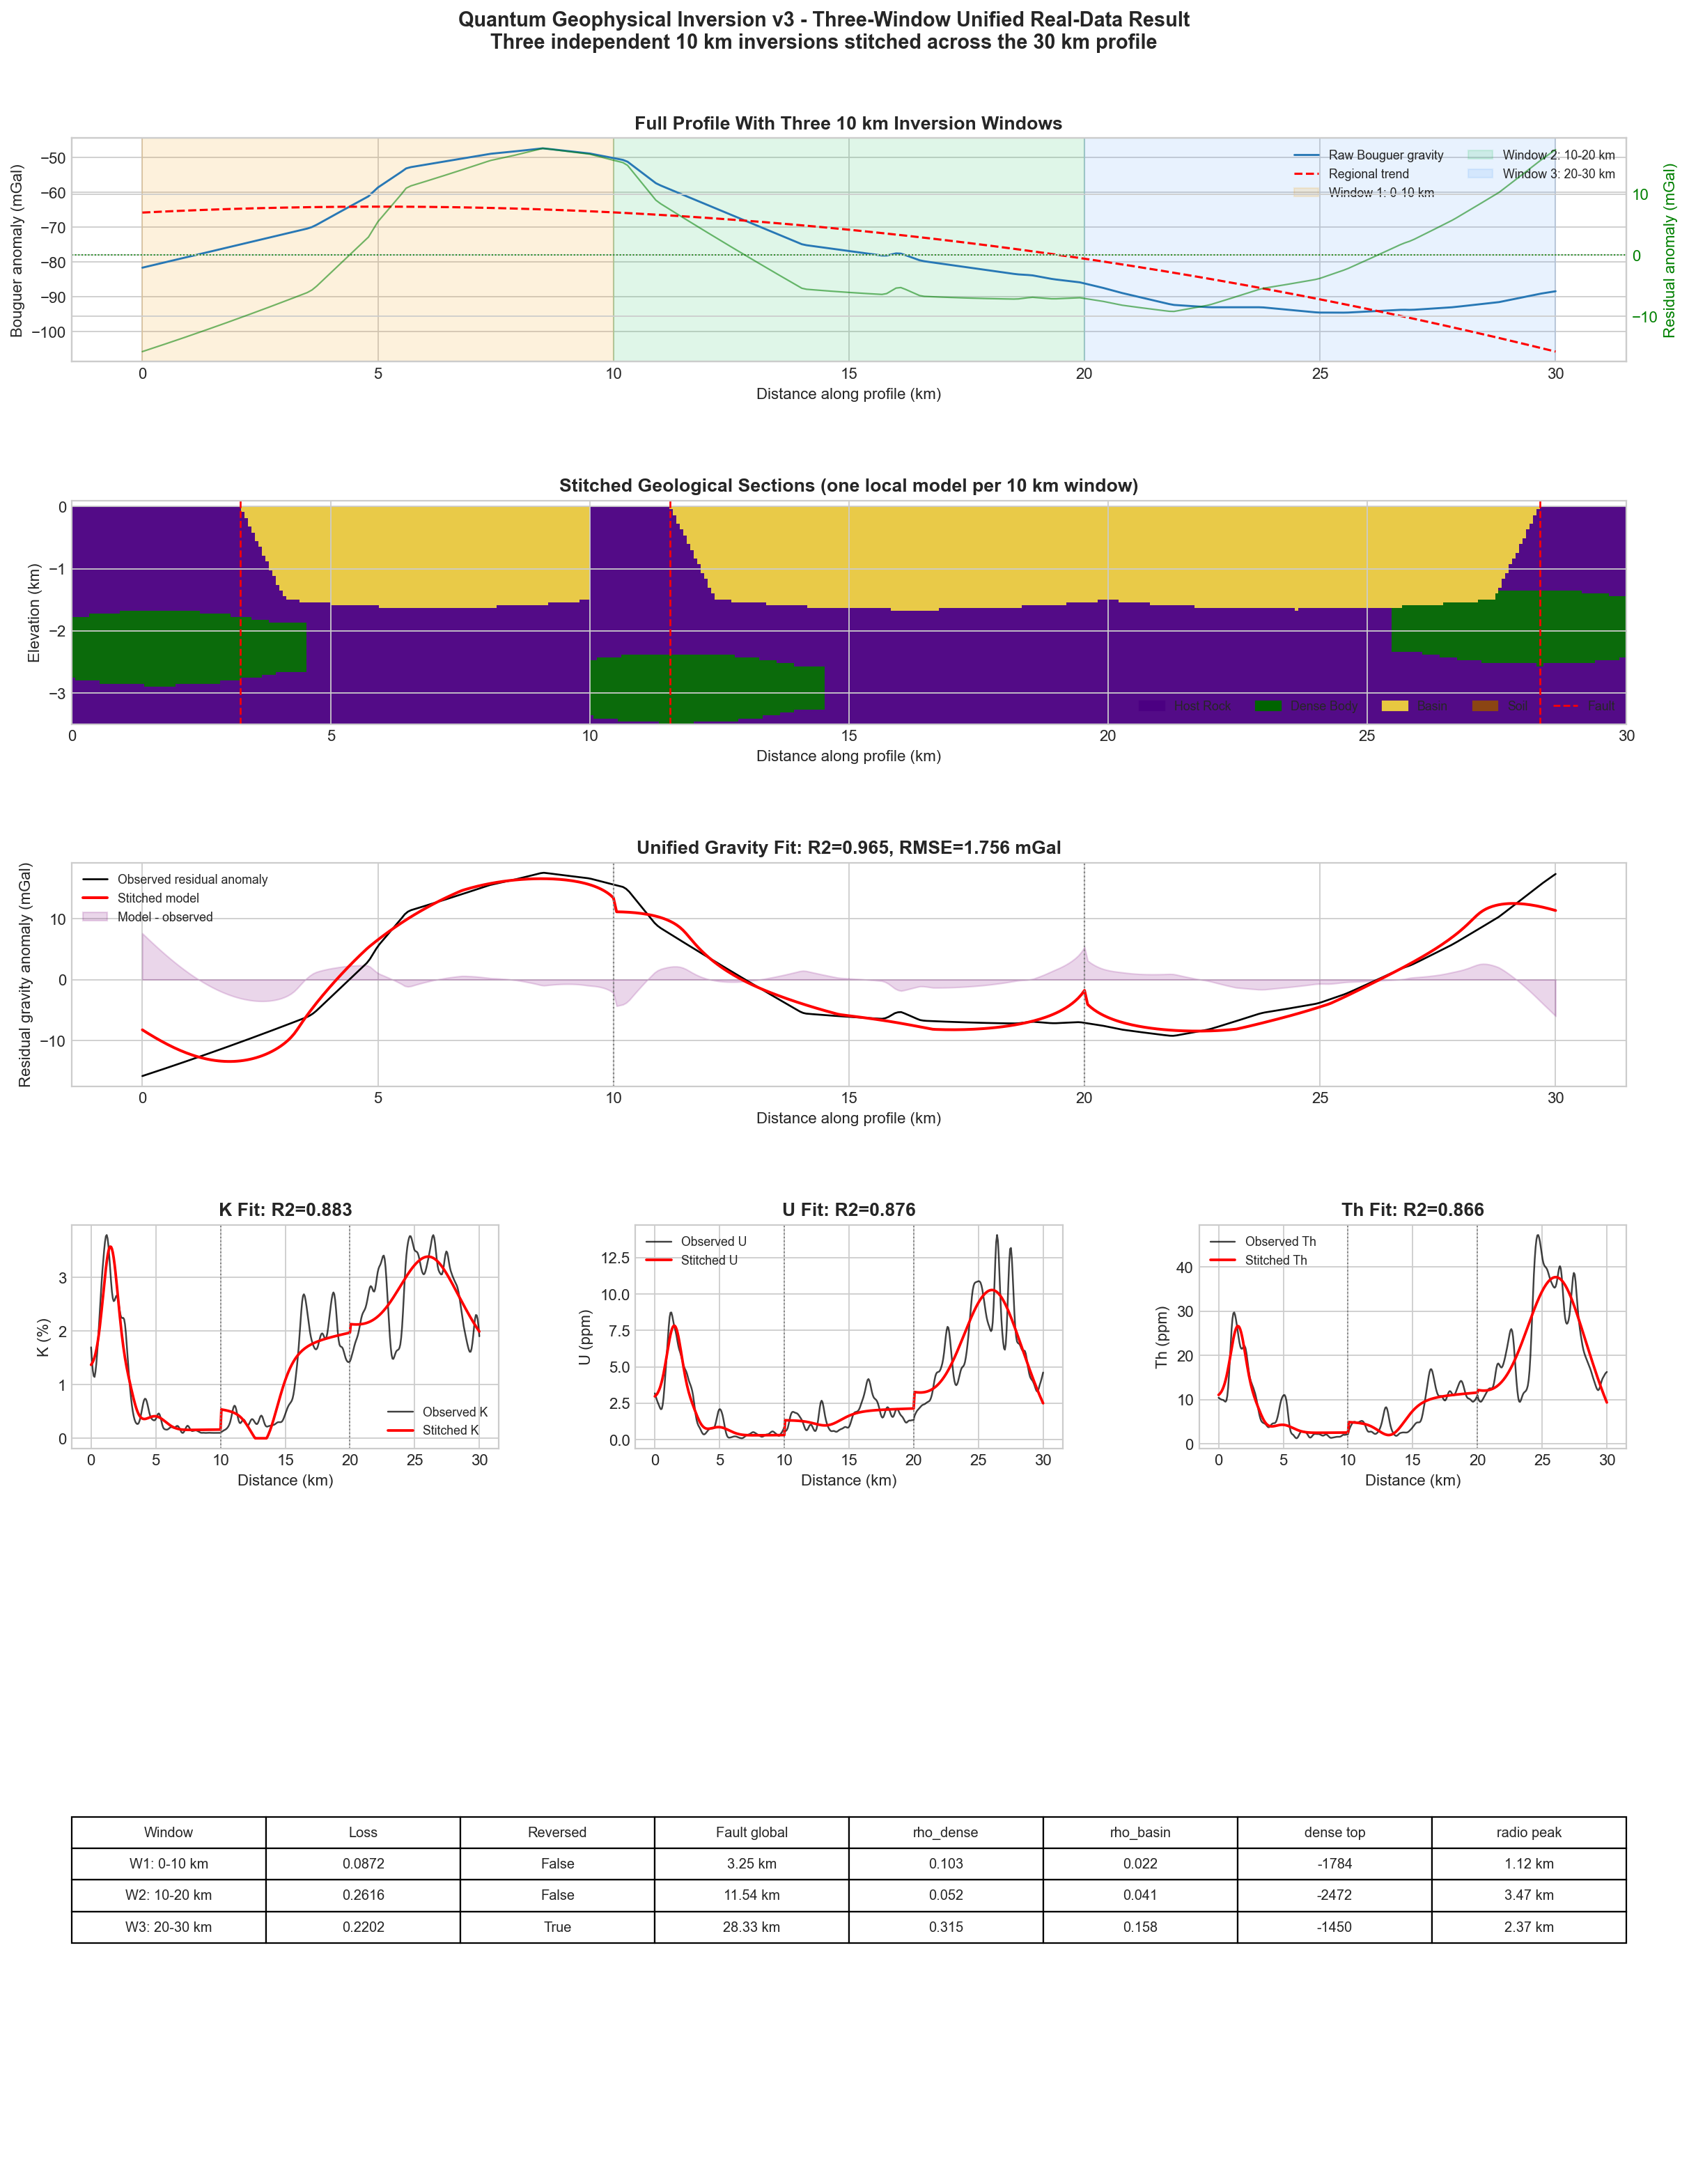
\includegraphics[width=\textwidth]{figures/stage3_unified_three_window_plot.png}
\caption{Complete Stage 3 full-profile stitched inversion result page.}
\end{figure}

\begin{figure}[H]
\centering
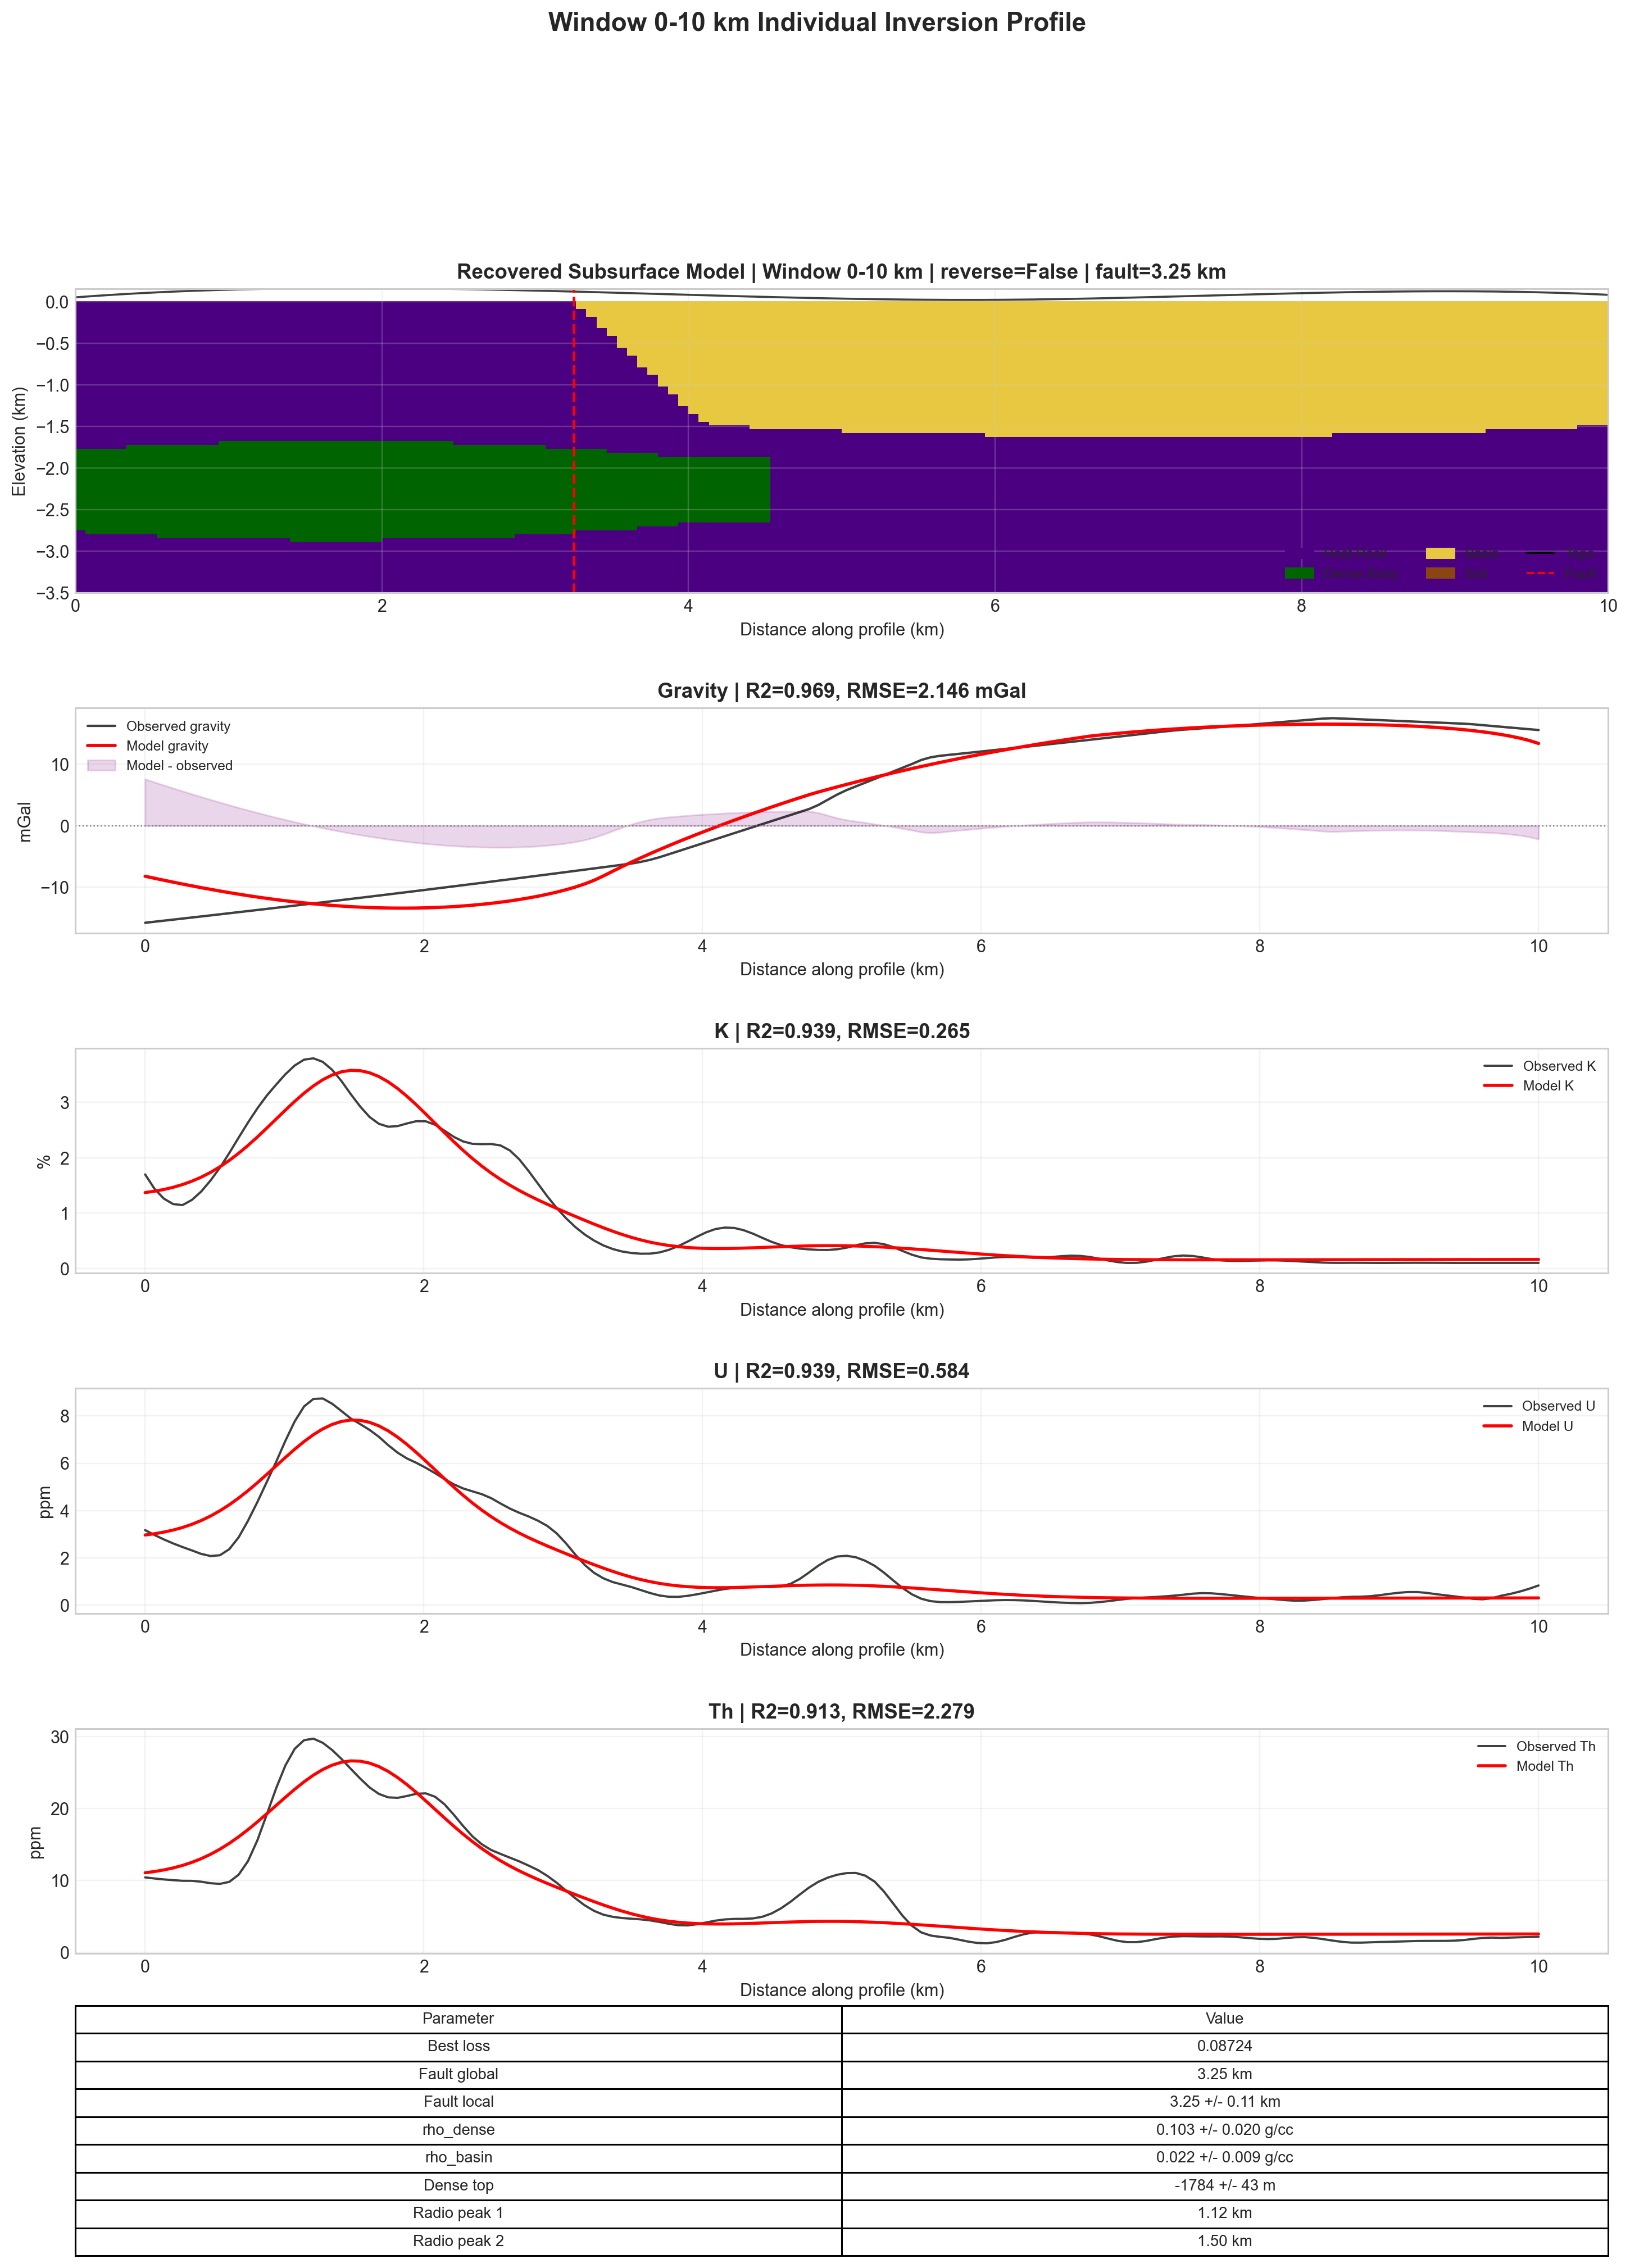
\includegraphics[width=\textwidth]{figures/stage3_window_00_10_individual_profile.png}
\caption{Complete individual inversion output for Window 1, 0--10 km.}
\end{figure}

\begin{figure}[H]
\centering
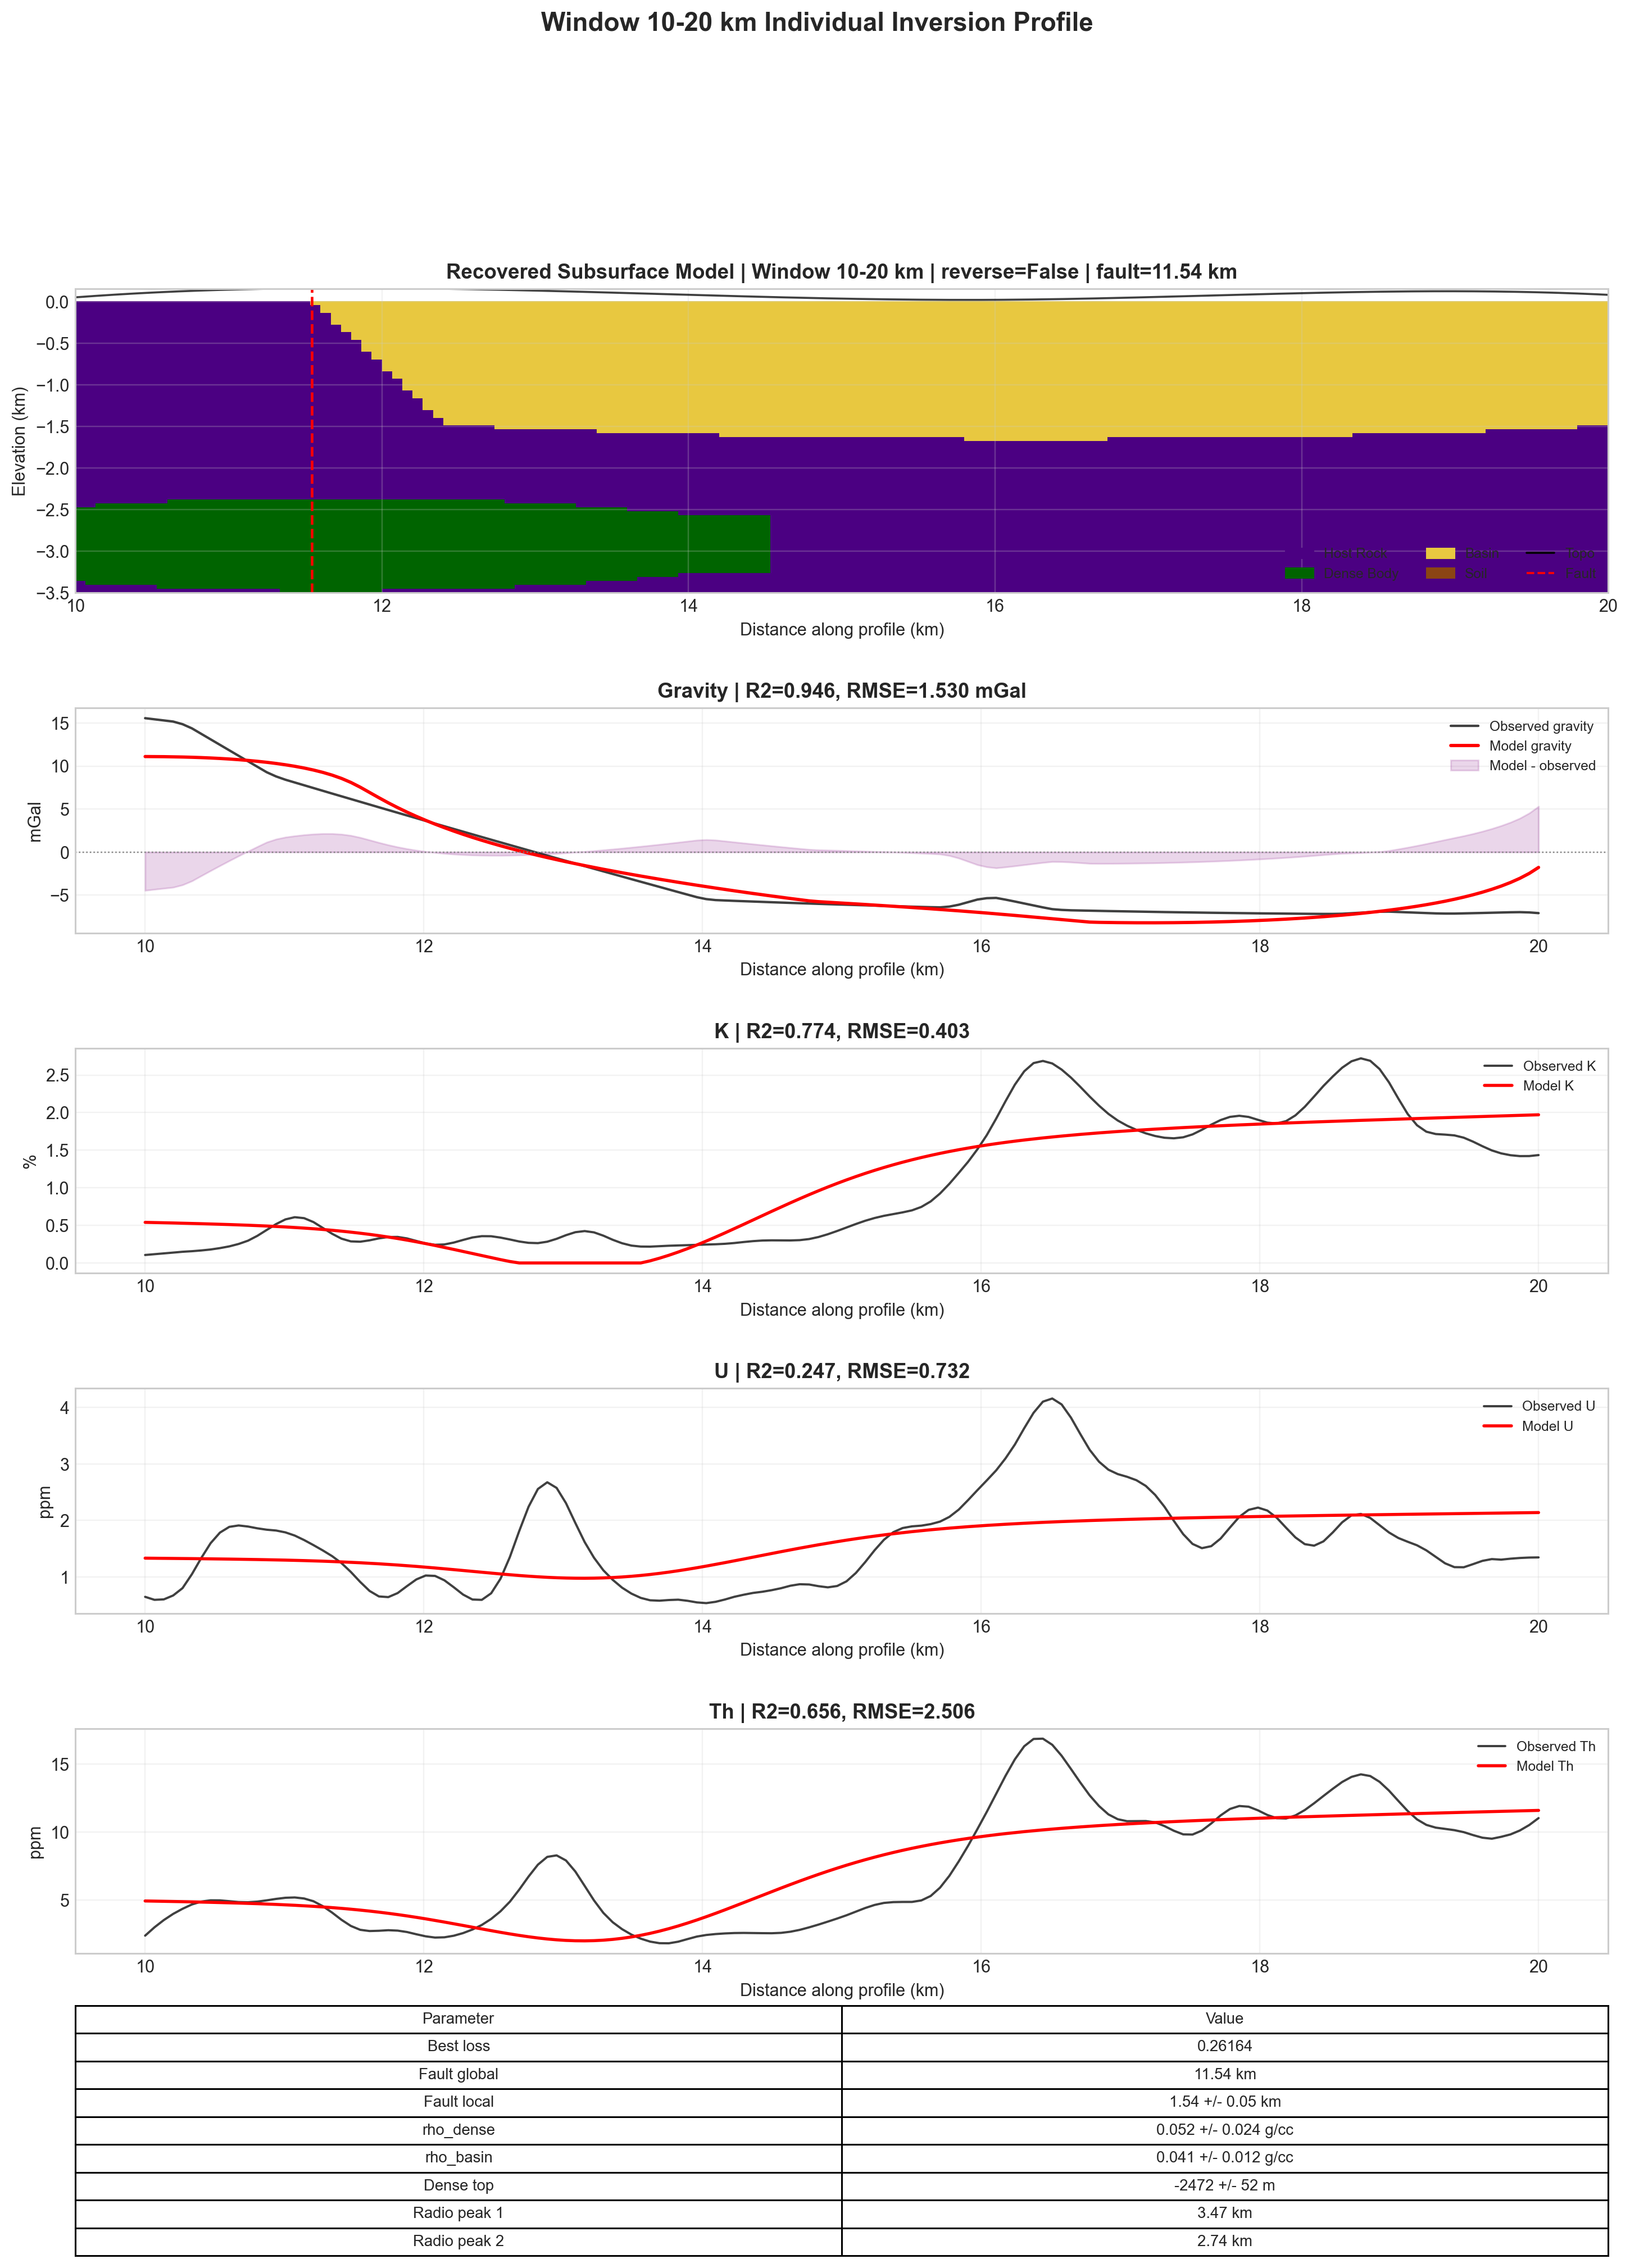
\includegraphics[width=\textwidth]{figures/stage3_window_10_20_individual_profile.png}
\caption{Complete individual inversion output for Window 2, 10--20 km.}
\end{figure}

\begin{figure}[H]
\centering
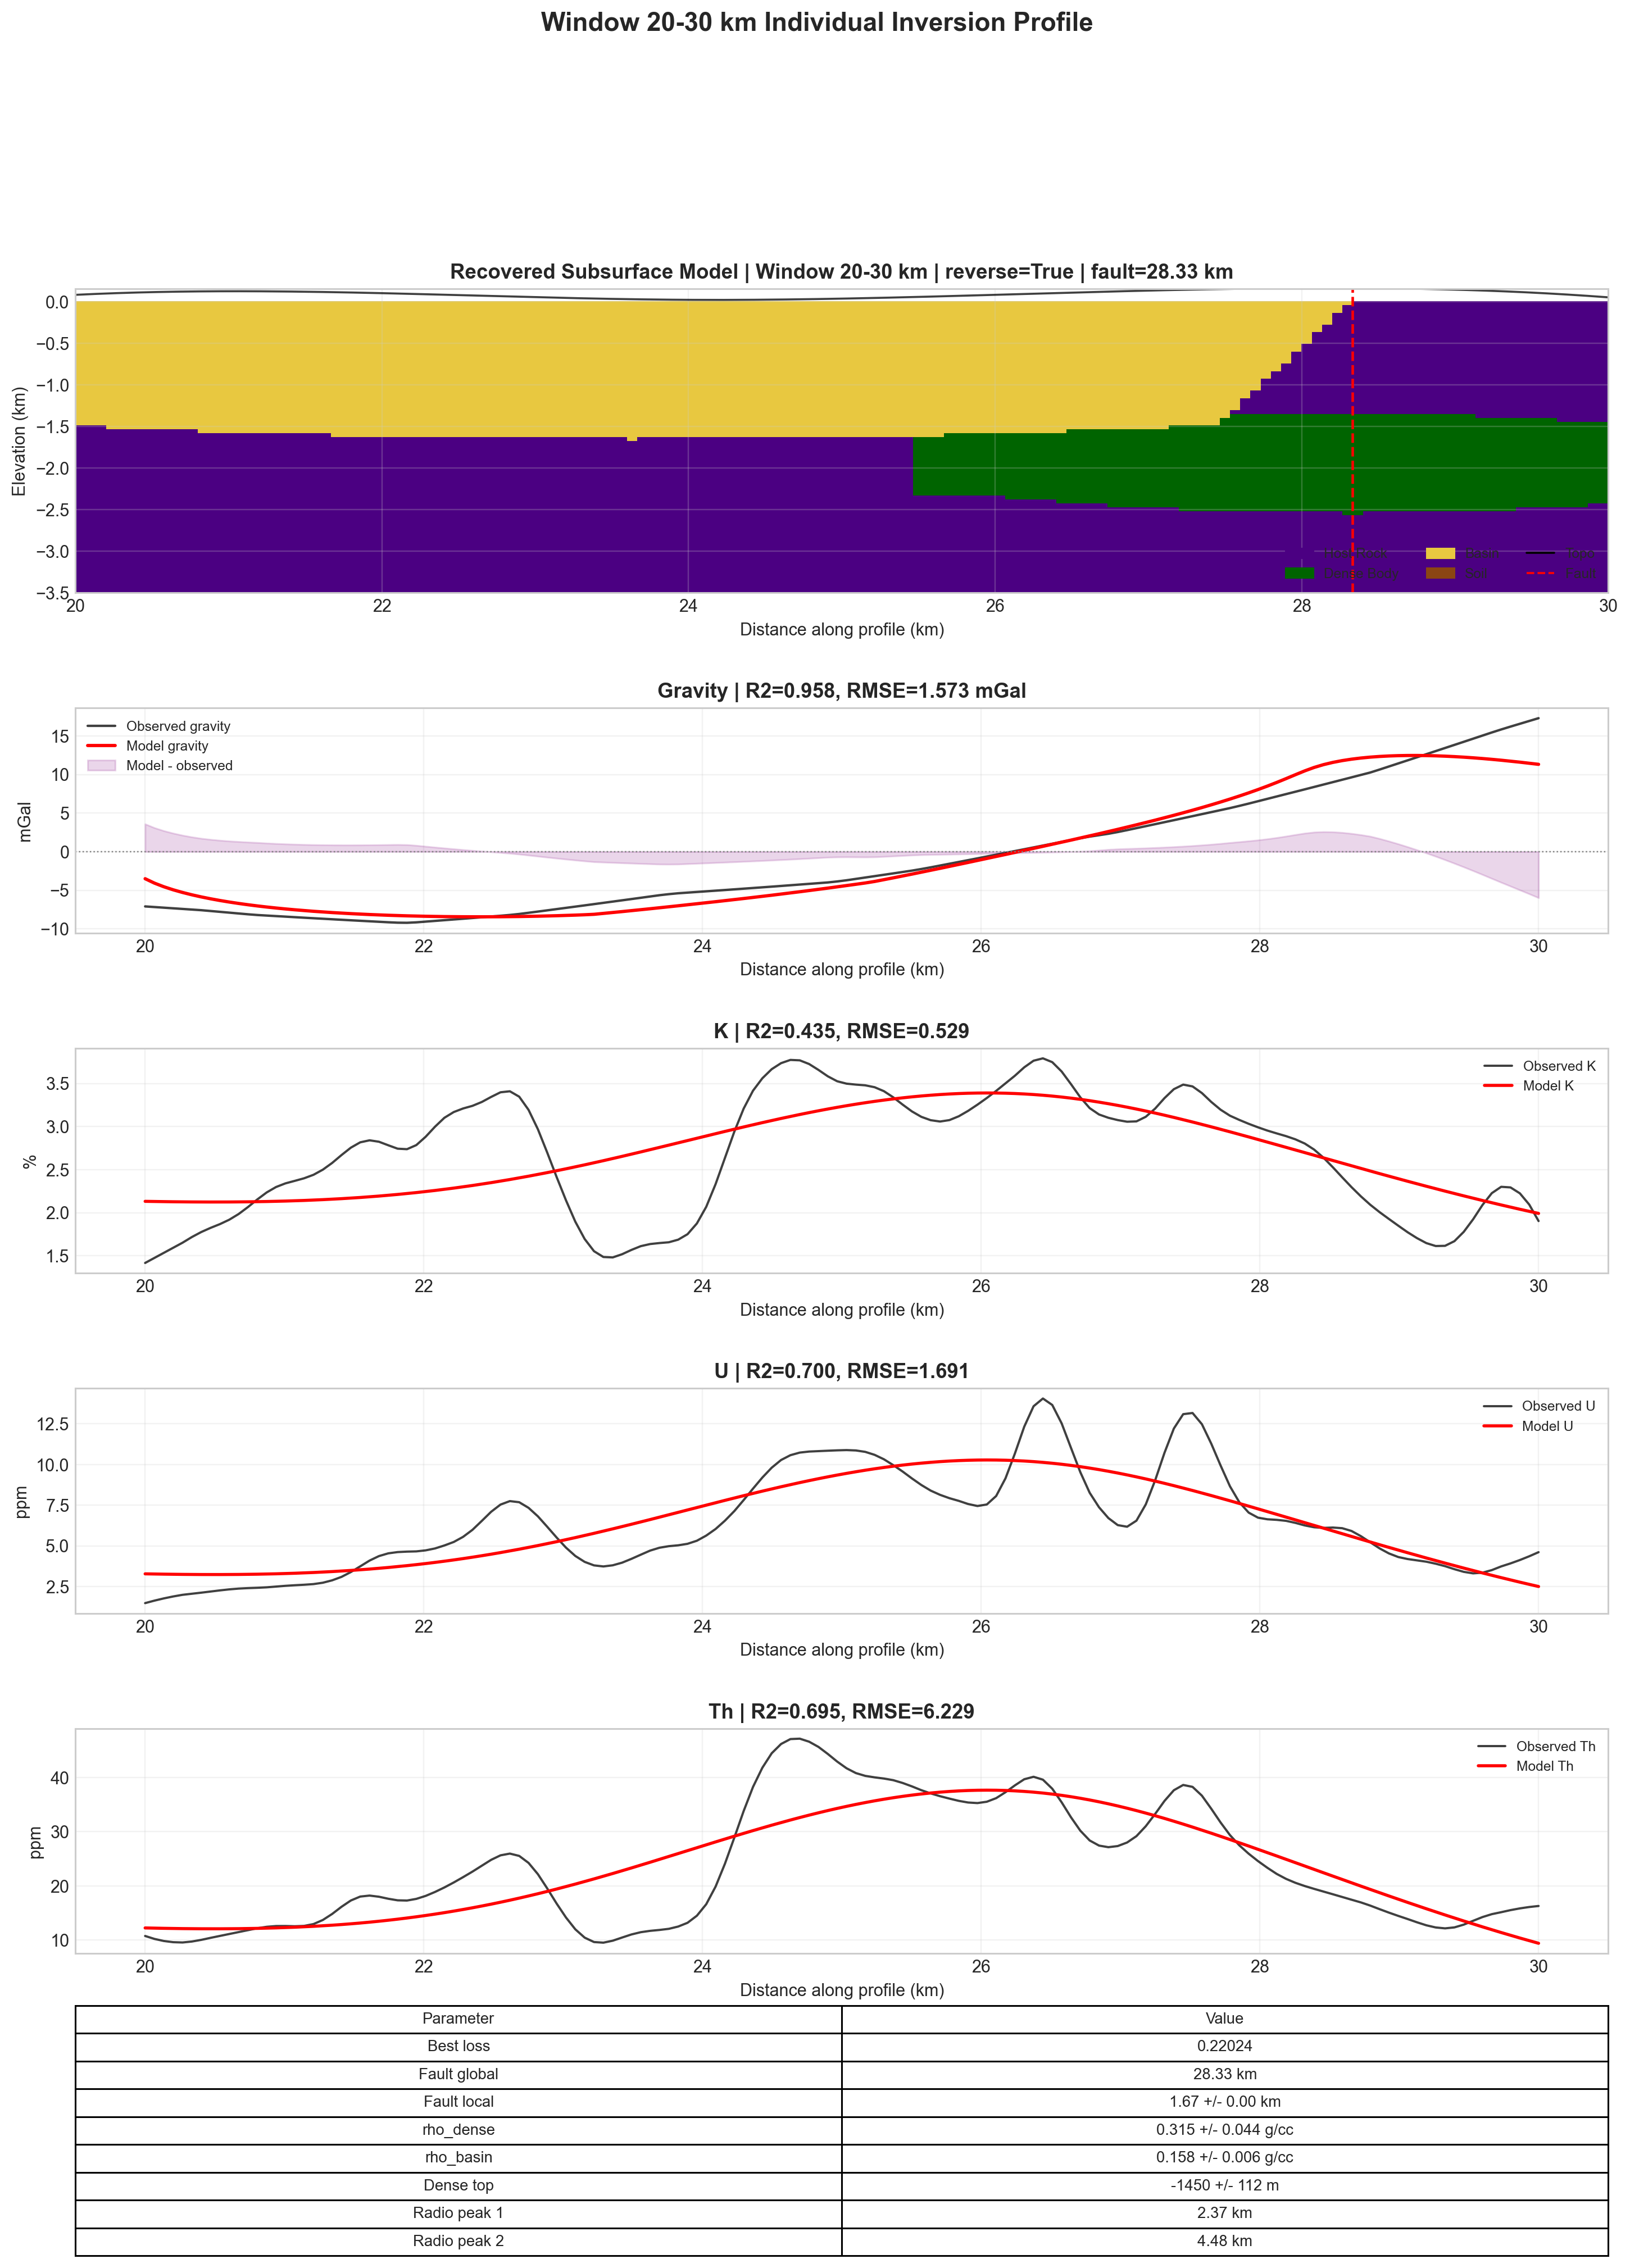
\includegraphics[width=\textwidth]{figures/stage3_window_20_30_individual_profile.png}
\caption{Complete individual inversion output for Window 3, 20--30 km.}
\end{figure}

\section{Computational Implementation}
\subsection{Folder Structure}
The final submission folder is organized as:
\begin{verbatim}
Quantum Inversion/
  00_Quantum_Regression/
  01_Model_Training_and_Forward_Modeling/
  02_Real_Data_Testing_10km_True_Inversion/
  03_Real_Data_Testing_Full_Profile_Three_Window_Stitched/
\end{verbatim}
Each stage contains source code, data or generated data, Slurm scripts where applicable, result plots, and summary files. Python cache files were removed from the cleaned submission copy.

\subsection{Param Shakti Execution}
The computationally heavier geophysical stages are designed for Param Shakti through Slurm scripts. The real-data jobs expose environment variables such as maximum iterations, population size, Monte Carlo sample count, and radiometric weight. The regression jobs are lightweight and self-contained; they use only NumPy and Matplotlib, and therefore do not require a quantum SDK installation. The synthetic quantum inversion uses PennyLane for the variational circuit and falls back from \texttt{lightning.qubit} to \texttt{default.qubit} when necessary.

\section{Discussion}
\subsection{Geophysical Interpretation}
The project demonstrates why direct transfer from synthetic to real geophysical data is not trivial. The synthetic model provides controlled validation, but real Bouguer gravity must be separated into regional and residual components before inversion. The sign of the residual may also be opposite to the synthetic convention, which is why negative gravity calibration scale is allowed. Radiometric behavior is even more survey-specific because K, U, and Th are shallow responses affected by soil, weathering, exposure, and local enrichment. The final real-data model therefore treats radiometric parameters as shallow surface-response shape controls rather than deep density parameters.

The 10 km real-data inversion is the most internally consistent result because it uses one local calibration and one local model. The full 30 km stitched result is broader and visually more complete, but it inherits boundary effects from independent windows. Its value lies in producing a unified profile-scale interpretation while preserving the validated 10 km inversion machinery.

\subsection{Quantum Interpretation}
The quantum regression stage shows how quantum expectation features can serve as a nonlinear basis for inverse modeling. The synthetic geophysical inversion goes further by using a variational quantum circuit as a parameter generator. The quantum circuit constrains the search to bounded physical ranges and provides a structured, entangled parameterization of the inverse problem. On present classical hardware this is a hybrid quantum-classical simulation, not a demonstrated quantum advantage. However, it establishes a reproducible pathway for later experiments with quantum kernels, variational quantum eigensolvers, amplitude encoding, or hardware-executed parameter proposal circuits.

\subsection{Limitations}
The main limitations are:
\begin{itemize}
    \item the gravity model is 2.5D rather than a fully 3D geological volume;
    \item density contrasts are effective calibrated contrasts, not direct petrophysical measurements;
    \item radiometric responses are modeled as shallow proxies rather than full radiation transport;
    \item the full 30 km interpretation is stitched from three independent windows;
    \item uncertainty is estimated by Monte Carlo perturbation around the final solution rather than full Bayesian posterior sampling;
    \item the current quantum computations are simulated on classical hardware.
\end{itemize}

\section{Conclusion}
This project successfully develops a staged quantum-assisted workflow for joint gravity and radiometric forward modeling and geophysical inversion. Stage 0 validates quantum feature-map regression on controlled linear and cubic datasets. Stage 1 validates the synthetic geophysical forward model and quantum-parameterized inversion with strong parameter recovery. Stage 2 adapts the workflow to real data through robust regional-trend removal, calibration, and real-style radiometric modeling, producing a high-quality 10 km inversion. Stage 3 extends the interpretation to the full 30 km profile using three stitched 10 km inversions and provides both unified and individual geological results.

The final deliverables include executable code, generated data, Slurm scripts for Param Shakti, publication-style result plots, and this Overleaf-ready report. The strongest scientific conclusion is that field geophysical inversion requires calibrated, survey-aware forward modeling; once this calibration is introduced, the quantum-assisted inversion framework can produce geologically interpretable and quantitatively strong results.

\clearpage
\bibliographystyle{plain}
\bibliography{references}

\end{document}

